%--------------------
% Packages
% -------------------
\documentclass[11pt,a4paper,notitlepage]{report}
\usepackage[utf8x]{inputenc}
\usepackage[T1]{fontenc}
\usepackage{mathptmx} % Use Times Font
\usepackage[pdftex]{graphicx} % Required for including pictures
\usepackage[pdftex,linkcolor=blue,pdfborder={0 0 0}]{hyperref} % Format links for pdf
\usepackage[all]{hypcap}
\usepackage{calc} % To reset the counter in the document after title page
\usepackage{enumitem} % Includes lists
\usepackage{titling}
\usepackage{xurl}
\usepackage[autostyle]{csquotes}
\DeclareQuoteStyle[quotes]{french}
  {\itshape\mkfrenchopenquote{\guillemotleft}}
  {\mkfrenchclosequote{\guillemotright}}
  {\itshape\textquotedblleft}
  {\textquotedblright}

\frenchspacing % No double spacing between sentences
\linespread{1.2} % Set linespace
\usepackage[a4paper, lmargin=0.1\paperwidth, rmargin=0.1\paperwidth, tmargin=0.08\paperheight, bmargin=0.09\paperheight]{geometry} %margins
%\usepackage{parskip}

\usepackage[all]{nowidow} % Tries to remove widows
\usepackage[protrusion=true,expansion=true]{microtype} % Improves typography, load after fontpackage is selected
\usepackage{indentfirst}
\usepackage{sectsty}
\usepackage{tikz}
\sectionfont{\fontsize{17}{15}\selectfont}

\usepackage{graphicx}
\graphicspath{ {./images/} }

\usepackage[square,numbers]{natbib}
\usepackage[center]{caption}

\title{How I Lost Faith in our Institutions}
\author{Jonathan B. A. Thorpe}

%-----------------------
% Set pdf information and add title, fill in the fields
%-----------------------
\hypersetup{ 	
pdfsubject = {},
pdftitle = {},
pdfauthor = {},
colorlinks = true,
urlcolor=[rgb]{0,0.5,0.5},
linkcolor=[rgb]{0,0.5,0.5},
citecolor=[rgb]{0,0.5,0.5}
}

\setlength{\parindent}{20pt}
\setlength{\parskip}{1em}


%-----------------------
% Begin document
%-----------------------
\begin{document} 

\begin{titlingpage}
\maketitle
\begin{abstract}
I am part of those who got away easy. The laptop class. Those who could stay working from home, my company was not in danger, I had a house and a garden. I used to believe that all this was inevitable, that we did our best. There were costly mistakes made along the way, but things were complicated. We locked down, we rolled out vaccines as soon as possible, and started pressuring people to take them. It was for the good of all. It was the only way. I was vaccinated like I felt I should. In the last four months I’ve changed. I think we could have done so much better, and when this all happens again we need to do better. I am now convinced that the COVID-19 pandemic has witnessed the most serious case of corporate misbehaviour backed by hijacked government institutions, health and scientific authorities, and the biggest propaganda machine ever seen on legacy and social media. Ordinary people have paid an unspeakable price which could have been mostly avoided if not for the profit driven agenda of the elites. I hope to convince as many as possible, in particular my peers, the privileged technologically and scientifically literate class, to reconsider their views if they are aligned with the mainstream narrative, to pierce the informational firewalls, look deeper and enforce change for the benefit of all. 
\end{abstract}
\end{titlingpage}

\section*{Background}

It started in the summer of 2021, I heard an \href{https://open.spotify.com/episode/7uVXKgE6eLJKMXkETwcw0D?si=AwYzUSIpRsGisRkZq_qQXw}{episode} of the Joe Rogan Experience with Bret Weinstein and Pierre Kory\footnote{Pierre Kory was the critical care service chief at the UW Health University Hospital (part of the University of Wisconsin School of Medicine and Public Health) until May 2020. He lost his job over his promotion of off-patent drugs for the treatment of COVID-19.} who were talking about repurposed drugs for prophylaxis and therapeutics, which supposedly had the power to end the pandemic whenever we chose to deploy it at scale. I was sceptical, surely we would have done it if we could. I put it in a corner of my mind. I’d been listening to Bret Weinstein speaking on a broad range of topics for a while, and he always impressed me with his refreshing combination of open mindedness and careful, serious scientific rigour. In a world which seemed to loose it’s grip his felt like a voice of reason, striking nuance between the extremes. After reading a number of articles which seemed to categorically discard Ivermectin as a potential help, I decided to forget about it. Even Merck who manufacture the drug said it didn’t work and warned against using it. Bret Weinstein could be wrong, like everyone, and on this one he probably was.

A few month later I heard that Oxford University had \href{https://www.bbc.com/news/health-57570377}{added Ivermectin to their PRINCIPLE trial}. I started wondering why, this drug which I’d read was not only useless in treating COVID-19, but was also dangerous and used as a horse dewormer would be investigated by extremely competent people. So I went back to the episode I heard, and listened to a few more episodes including \href{https://open.spotify.com/playlist/0ZCLBEbktYqp1lSheZS81E?si=5ad3d9f833804821}{Robert Malone}\footnote{See Robert W Malone's scientific credentials on his \href{https://scholar.google.com/citations?user=Jf1bApYAAAAJ&hl=en}{Google Scholar profile}, he holds nine patents on mRNA vaccine technology and has raised concerns on their safety. He has strongly promoted the use of off-patent drugs for the treatment of COVID-19.} and \href{https://open.spotify.com/episode/0aZte37vtFTkYT7b0b04Qz?si=a1uycZk4RduXt09K0sHPng}{Peter McCollough}\footnote{See Peter A McCullough's scientific credentials on his \href{https://scholar.google.com/citations?hl=en&user=LzqEaOkAAAAJ}{Google Scholar profile}, he is a board-certified cardiologist who has testified before committees of the US and Texas Senates regarding the patient treatment of COVID-19 using off-patent drugs.}. These people were described by the mainstream media as spreading misinformation and yet seemed extremely intelligent, well meaning and could not have been more qualified. So I decided to start systematically fact checking them, as well as the dominant narratives. It was quite a ride, and overall they have proved to be the most valuable source of information I’ve had throughout this pandemic. I do not see them as a source of truth but a source of leads. The information is there, if you know where to look. Once you see the pattern emerging, you cannot look away. 

When I tried to discuss these facts around me, I was predominantly met by a form of visceral inhibitory mechanism which I expect is common in authoritarian regimes. Exchanges became instantly heated and unproductive. My sources were diffuse, long form podcasts, hearings held by senators, emotional testimony from highly qualified doctors, scientific articles, world press and statistics and I couldn't hope to do them justice in casual conversation. Few would believe that our mainstream sources would deceive us so profoundly. So I decided to go for a relatively short highly referenced document. I take no credit in unearthing these elements of information, my aim is condense them into a form which is more digestible, so as to attempt to unveil their global coherence.

\section*{The only solutions were the ones we were allowed}

It was early 2020, the waves were coming, people panicked. Hospitals were getting overloaded with people who were struggling to breathe, they needed ventilators, they were dying. There was a rush to find effective treatments and therapeutics, mountains of data from around the world was pouring in with many promising leads. The decisions however were not to be influenced by physicians in hospitals and clinics who knew this new disease better than anyone. Instead they were made by a handpicked few, with strong ties to the pharmaceutical industry\footnote{In COVID-19 Treatment Guidelines Panel Financial Disclosure for Companies Related to COVID-19 Treatment or Diagnostics \cite{nihTreatmentPanelFinancialDisclosure}, \textit{Gilead} (behind Remdesivir) appears 7 times, \textit{Pfizer} 3 times, \textit{Merck} 7 times, \textit{AstraZeneca} 3 times. In France the influence of Big Pharma in validating Remdesivir was also clear \cite{doi:10.1177/1440783320936740}, \cite{mediapart31032020}}. The bar for recommendation was set. It was to be large centralised randomised double blind trials, not accumulated experience by people on the front line.

%https://pubmed.ncbi.nlm.nih.gov/33340409/

These large trials are \href{https://www.sofpromed.com/what-is-the-cost-of-a-clinical-trial}{expensive}, tens of millions of dollars. The only entities capable of running them  fast enough were corporate pharmaceutical giants with obvious conflicts of interest. Remdesivir won the race after mediocre results and an \href{https://blogs.bmj.com/bmj/2020/06/10/remdesivir-in-the-plague-year-observations-of-the-most-remarkable-occurences/}{endpoint change} mid way through a trial \cite{bmj10062020} which was funded by tax payer money for private benefits. Safety protocols were short circuited and an \href{https://www.science.org/content/article/very-very-bad-look-remdesivir-first-fda-approved-covid-19-drug}{unjustifiable emergency use authorisation} was given by the FDA \cite{science28102020} which receives \href{https://today.uconn.edu/2021/05/why-is-the-fda-funded-in-part-by-the-companies-it-regulates-2/#}{45\% of its funding} from the industry it is meant to regulate \cite{uconn21052021}. It was then enforced as the recommended treatment with a price tag of \href{https://www.ajmc.com/view/gilead-sciences-sets-us-price-for-covid19-drug-at-2340-to-3120-based-on-insurance}{thousands of dollars} per patient \cite{ajcm20062020}. Physicians across the US and much of the western world had their hands tied by central medical authorities and piloting committees. Remdesivir became the official protocol, those who deviated risked disciplinary action.

We briefly heard about vitamin D, hydroxychloroquine, ivermectin and many other potential avenues of investigation, but these were quickly and neatly tidied up by invisible forces. They were systematically discarded, debunked and their proponents were paraded as clowns, lunatics, conspiracy theorists, right wing extremists. No large government funded trials or shortcuts and exceptions for them, only corporate sponsored scientific scepticism and journalistic derision resulting in public indifference. Any solution would need to be new and above all, profitable. Our arsenal of public domain tools were declared useless. There were no monthly reviews of medical evidence from people on the front line, just death counts and prayers.

Remdesivir, despite its huge price tag and intravenous administration, \href{https://www.thelancet.com/journals/laninf/article/ PIIS1473-3099(21)00485-0/fulltext}{didn’t significantly reduce mortality} (\cite{Ader21}, \cite{Yan2021-pc}). It was time for the main event. Vaccines. The deciders had already planned their mass vaccination pandemic response in detail two years before the start of the pandemic, with \href{https://cepi.net/news_cepi/global-partnership-launched-to-prevent-epidemics-with-new-vaccines/}{CEPI}, backed by the Bill and Melinda Gates Foundation and the firepower of the World Economic Forum\footnote{The World Economic Forum, which is mostly funded by its 1,000 member companies (typically global enterprises with more than five billion US dollars in turnover) as well as public subsidies, views its own mission as \textit{improving the state of the world by engaging business, political, academic, and other leaders of society to shape global, regional, and industry agendas}. Big tech, pharma, media, they are all \href{https://www.weforum.org/partners}{partners} there. Many top politicians have been through their \href{https://www.informedchoiceaustralia.com/post/wef-and-their-young-global-leaders-program}{Young Global Leaders} program \cite{ica09122021}.}. Their \href{https://www.who.int/medicines/ebola-treatment/TheCoalitionEpidemicPreparednessInnovations-an-overview.pdf}{business plan}, masqueraded as philanthropy in a presentation to the WHO in July 2017 \cite{cepi072017} had already sorted how vaccine developers would be shielded from liability (see Figure \ref{fig:CEPI-slide-10}), would suffer no economic cost and would reap all the benefits of state sponsored research (see Figure \ref{fig:CEPI-slide-6}). They had already identified coronaviruses as prime targets (see Figure \ref{fig:CEPI-slide-9}) for profitability and established that the WHO would act as \textit{normative} lead agency (see Figure \ref{fig:CEPI-slide-19}), with massive private investment from the Bill and Melinda Gates Foundation\footnote{To ensure the WHO could properly enforce its normative role, the Bill and Melinda Gates Foundation have become it's second largest contributor after the UK (the US which was its largest pulled out under Trump). Its third largest contributor is the \href{https://en.wikipedia.org/wiki/GAVI}{GAVI} vaccine alliance (which is a proxy for the Bill and Melinda Gates Foundation, its second largest contributor)}.

When COVID-19 came the plan sprung into action, it was a golden opportunity for a massive return on corporate CEPI investment. Pesky physicians successfully experimenting with repurposed, cheap, highly safe and available off-patent drugs and nutritional supplements were a risk, a hindrance, and were erased using any means necessary. It was essential that no viable alternatives emerged in order for emergency use authorisations to be granted\footnote{The FDA \href{https://www.fda.gov/emergency-preparedness-and-response/mcm-legal-regulatory-and-policy-framework/emergency-use-authorization}{states} that it \textit{may authorise unapproved medical products or unapproved uses of approved medical products to be used in an emergency to diagnose, treat, or prevent serious or life-threatening diseases or conditions caused by CBRN threat agents when certain criteria are met, including there are no adequate, approved, and available alternatives.} \cite{fda-eua}}. We waited for our saviours to develop the vaccines in our domestic prison cells, while millions died. Tax payer money funding for private profits and in addition to having \href{https://www.cnbc.com/2020/12/16/covid-vaccine-side-effects-compensation-lawsuit.html}{no liability} for adverse effects \cite{cnbc17122020}, governments around the world would enforce their use, pressured by the WHO. A corporate paradise. Safety procedures were short circuited again. Pfizer were given emergency use authorisation by the FDA (without releasing the trial data) and were given immunity by the government despite having one of the \href{https://www.ncbi.nlm.nih.gov/pmc/articles/PMC2875889/}{worst records} in fraud and corruption in the pharmaceutical industry \cite{evans052010}, including the largest \href{https://www.justice.gov/opa/pr/justice-department-announces-largest-health-care-fraud-settlement-its-history}{fraud settlement} in history in 2009 \cite{pfizer-fraud-settlement}. Citizens were given the choice between self imprisonment, triweekly punitive nose rape or experimental vaccines. Workers, including exhausted front line medics were faced with obligatory vaccination or starvation. People started policing each other. We needed the boosters, and super boosters, adolescents, children. One. single. solution.

Lockdowns came, then came again, wave after wave. The vaccines didn't stop transmission. Small businesses died, restaurants and shops closed, domestic abuse rocketed, children couldn't play, learn or see adult faces, the poor suffered most, while big tech, big pharma, big distribution pocketed the billions, people turning to Meets, Zoom, Facebook, Amazon, Walmart\footnote{By October 2020, 40 million Americans filed for unemployment during the pandemic, but billionaires saw their net worth increase by half a trillion dollars \cite{businessinsider30102020}}. The biggest upward transfer of wealth in the history of humankind \cite{oxfam17012022}. Mounting evidence against systematic repeated total vaccination and lockdowns and any information which could lead to scepticism was systematically classified as \textit{mis}information by mainstream and social media platforms. Whether they were true or not was irrelevant. Truth was redefined, vaccines and lockdowns were the only truth. Self organised groups with hundreds of thousands of adverse effect sufferers were disappeared from social media. Crushing evidence from around the world and our own databases, scientists and doctors, censored and firewalled to ensure compliance, the mainstream profit driven narrative hammered into our heads wherever we looked. We were going to get the vaccines and lockdowns, the only solutions we were allowed.

\section*{Tales from around the world}

While we were busy worrying about when the vaccines would finally save us, elsewhere around the world people knew they could only count on themselves. They could, of course, also count on the WHO and the FDA to spread their corporate driven Remdesivir recommendations and vaccine fanaticism with great effect, but by September 2021 \href{https://www.nature.com/articles/d41586-021-02383-z}{less that 1\%} of lower income countries had been fully vaccinated \cite{nature15092021}. Some CEPI principles (see Figure \ref{fig:CEPI-slide-6}) were seemingly secondary. Uttar Pradesh (the most populous state in India\footnote{Uttar Pradesh has a population of 240 million. If it was a country it would be the 5th most populous in the world.}) replicated results from numerous small scale studies showing outstanding results for prophylactic Ivermectin\footnote{According to the \href{https://indianexpress.com/article/cities/lucknow/uttar-pradesh-government-says-ivermectin-helped-to-keep-deaths-low-7311786/}{Uttar Pradesh State Surveillance Officer} Vikssendu Agrawal \cite{indianexpress12052021} \textit{In May-June 2020, a team at Agra, led by Dr Anshul Pareek, administered Ivermectin to all RRT team members in the district on an experimental basis. It was observed that none of them developed Covid-19 despite being in daily contact with patients who had tested positive for the virus.}} and Vitamin D and decided to base their approach on these results using targeted med-kits for positive tests and contact cases (the \href{https://www.aiims.edu/en.html}{AIIMS} lent their \href{https://www.cureus.com/articles/64807-prophylactic-role-of-ivermectin-in-severe-acute-respiratory-syndrome-coronavirus-2-infection-among-healthcare-workers}{support} \cite{Behera2021-qu}). Their government \href{https://indianexpress.com/article/cities/lucknow/uttar-pradesh-government-says-ivermectin-helped-to-keep-deaths-low-7311786/}{declared} that this helped them keep mortality down to an astounding extent \cite{indianexpress12052021}. They were \href{https://www.who.int/india/news/feature-stories/detail/uttar-pradesh-going-the-last-mile-to-stop-covid-19}{praised by the WHO} \cite{who07052021} who referred to their med-kits without referring to what was inside \cite{medicalupdateonline21052021} \cite{hindu14092020}, presumably because it went against their \href{https://www.who.int/news-room/feature-stories/detail/who-advises-that-ivermectin-only-be-used-to-treat-covid-19-within-clinical-trials}{own recommendations}. Although Uttar Pradesh is slightly less vaccinated and nearly three times more densely populated than the second most populous state in India (Maharashtra), their mortality rate is \hyperref[fig:india-stats]{13 times lower} overall and has been throughout the pandemic (see Figures \ref{fig:india-stats}, \ref{fig:india-uttarpradesh-mortality}, \ref{fig:india-maharashtra-mortality}). They have essentially flattened COVID-19 \cite{hindustantimes19092021}. This was not considered worth any attention by our scientific, pharmaceutical, media and governmental institutions, rare mainstream media coverage focused on baselessly discrediting Ivermectin \cite{torontoStar28012022}.

Elsewhere in India, the two states of Uttarakhand and Kerala gave us a natural experiment of unusual magnitude. Uttarakhand decided to deploy prophylactic Ivermectin as a response to the Delta wave in may 2021 \cite{economictimes12052021}, their daily mortality went down to zero within two month and has essentially stayed there ever since (see Figure \ref{fig:india-uttarakhand-mortality}). Kerala conversely was using \href{https://dhs.kerala.gov.in/wp-content/uploads/2021/04/Kerala-State-COVID-19-guidelines-Version-3.pdf}{generic drug and supplement cocktails} up to summer 2021 \cite{keralagov24042021} to great effect, when they succumbed to pressure from the WHO in the middle of the Delta wave. They dropped their protocol\footnote{According to The Hindu \cite{hindu06082021} \textit{The new protocol has removed drugs like Ivermectin, Favipiravir, and Hydroxychloroquine that were not really supported by evidence; Remdesivir has been retained on the basis of emergency use authorisation;}} in favour of the expensive and ineffective Remdesivir \cite{hindu06082021}. Their mortality rate has exploded and remained extremely high ever since (see Figure \ref{fig:india-kerala-mortality}). The WHO didn't consider their recommendation might have been a factor.   

Peru offered another large scale \href{ https://osf.io/9egh4/}{real world experiment} in ivermectin deployment \cite{Chamie2021}. The mortality for over 60 year olds was cut 14 fold in three month after the introduction of ivermectin, then jumped back up 13 fold once the new president restricted its use (see Figure \ref{fig:peru-mortality}). Per state analysis for 25 states showed the effects to be tied to deployment date and quantity with a very high significance (see Figure \ref{fig:peru-operation-mot}). Africa, where a number of countries have been using ivermectin systematically for over 35 years\footnote{Ivermectin is widespread use across Africa notably thanks to Merck's \href{https://www.merck.com/stories/mectizan/}{Mectizan Donation Program} \cite{merck06012021}} to treat an array of different tropical diseases to great effect provided an accidental demonstration of its effectiveness against COVID-19. Based on a \href{https://www.medrxiv.org/content/early/2021/03/26/2021.03.26.21254377.full.pdf}{comparative study}\footnote{\citet{Tanioka2021.03.26.21254377} showed an average COVID mortality of 14.4 per million in African countries which use ivermectin while African countries which don't have an average mortality rate of 129.1 per million (9 times higher)} of African state which used and didn’t use ivermectin for treating other illnesses \cite{Tanioka2021.03.26.21254377}, the chairman of the Tokyo Metropolitan Medical Association decided to \href{https://www.tokyo-np.co.jp/article/123988}{allow physicians to use ivermectin off label} \cite{tokyoweb13082021} (while not officially recommending it as it would be in direct defiance of the WHO recommendations) to deal with an uncontrollable situation. All around the world, using cheap repurposed drugs, states, provinces and countries defied the WHO and obtained results which western countries could only dream of. None of this was reported. Ultra qualified physicians were screaming for these drugs to be allowed and were cancelled and harassed by the authorities. Many lost their licenses. 

\section*{Misinformation works best when it comes from above}

The narrative surrounding the pandemic has been relentlessly hammered into our minds throughout the passed two years. Using carefully selected informational emphasis and systematic censorship, demonisation and ridicule of dissent our institutions have imposed lockdowns and vaccination to the people. This has been remarkably effective, but cracks have started to appear. The narrative has shown itself to be paper thin to anyone who cares to look for themselves. A few case studies of systemic top-down misinformation.

\subsection*{Hydroxychloroquine}

The use of hydroxychloroquine for the treatment of COVID-19 was \href{https://pubmed.ncbi.nlm.nih.gov/32205204/}{investigated} in early 2020 by a team led by Didier Raoult\footnote{See Didier Raoult's scientific credentials on his \href{https://scholar.google.fr/citations?user=n8EF_6kAAAAJ&hl=fr}{Google Scholar profile}. He is one of the top virologists in the world and has a history of resisting big pharma and exploring off-patent alternatives \cite{doi:10.1177/1440783320936740}.} following some signs of effectiveness against the original SARS and in early Chinese studies \cite{Lagier2020-dw}. Many other studies followed showing mixed results with a high sensitivity to COVID-19 development stage and dosage. However it's effectiveness when used appropriately has been \href{https://www.ncbi.nlm.nih.gov/pmc/articles/PMC8023208/}{confirmed} by a number of large studies of clinical outcomes \cite{Mokhtari2021-ot}. 

%https://www.legifrance.gouv.fr/jorf/id/JORFTEXT000041400024


The WHO were meant to perform hydroxychloroquine trials in 2020, but a series of anomalies occurred. The trials were \href{https://www.theguardian.com/world/2020/may/25/who-world-health-organization-hydroxychloroquine-trial-trump-coronavirus-safety-fears}{put on hold} amid safety fears in light of a paper published in the Lancet that showed people taking hydroxychloroquine were at higher risk of death and heart problems than those who were not \cite{guardian25052020} . A few weeks later the Lancet \href{https://www.theguardian.com/world/2020/jun/04/covid-19-lancet-retracts-paper-that-halted-hydroxychloroquine-trials}{retracted the paper} \cite{guardian03062020} after the study was shown to be \href{https://www.theguardian.com/world/2020/jun/03/covid-19-surgisphere-who-world-health-organization-hydroxychloroquine}{completely fraudulent} \cite{guardian03062020b}. The WHO trials were resumed but it surfaced that the dosage which were used were \href{https://www.francesoir.fr/politique-monde/oxford-recovery-et-solidarity-overdosage-two-clinical-trials-acts-considered}{borderline lethal} \cite{francesoir25062020}. The Indian Council of Medical Research (ICMR) wrote to the WHO expressing concerns with the dosages used \cite{newindianexpress29052020}, which were four times higher than the ones they were successfully using. Maybe the WHO, with the Bill and Melinda Gates Foundation as its second highest contributor\footnote{The WHO \href{https://www.who.int/about/funding/contributors}{top contributors} \cite{who-contributors2020} were the US, UK and the Bill and Melinda Gates Foundation for 2018-2019, but the US stopped its funding}, could have been compromised by conflicts of interests\footnote{The Bill and Melinda Gates Foundation have a 100 million dollar investment in CEPI who had set the terms for vaccine profit returns in 2017 (see Figure \ref{fig:CEPI-slide-6})}. Interestingly the current world usage of hydroxychloroquine for the treatment of COVID-19 seems to be an inverse function of WHO influence (see Figure \ref{fig:hydroxychloroquine-countries}).


\subsection*{Ivermectin}

Ivermectin has been widely used in humans since 1987 with an exceptional safety record (\cite{Smit2016-fq}, \cite{Crump2011-ev}). It won its inventor the Nobel Prize and is on the WHO’s list of essential medicines \cite{Crump2017-qg}. It has essentially eradicated a number of tropical diseases in Africa, and was so effective, cheap and safe that Merck created a large scale \href{https://www.merck.com/stories/mectizan/}{donation program with over 4 billion doses distributed over 35 years} \cite{merck06012021}. Presumably they didn't think it was dangerous until COVID-19 hit and then changed their minds despite \href{https://academic.oup.com/ofid/article/8/Supplement_1/S365/6450290}{studies} \cite{wentzel2021} confirming the absence of adverse effects for treating it\footnote{One might think that Merck might be deliberately downplaying Ivermectin in favour of Molnupiravir which sells  for \$700. \href{https://www.bloomberg.com/news/articles/2021-12-08/merck-s-mrk-covid-pill-must-first-overcome-anti-vax-ivermectin-misinformation}{Conspiracy theory} of course.}. It was identified as an extremely promising prophylactic and therapeutic for COVID-19 early on and many \href{https://c19ivermectin.com/}{preliminary studies} suggested very high effectiveness. These never translated into the large scale RCT necessary for wide scale adoption. The resulting scientific uncertainty was pushed hard to discourage further interest and drive proponents to the fringes (\cite{bbc06102021}, \cite{guardian13092021}, \cite{guardian24092021}, \cite{guardian24092021b}). Proponents \href{https://bird-group.org/the-bbcs-recent-article-false-science-is-disintegrating-under-scrutiny/}{defended themselves}, but no one heard. Papers reporting large scale effects in test runs have been pulled based on \href{https://healthpolicy-watch.news/mexico-city-officials-in-row-over-misleading-paper-to-justify-its-ivermectin-drive/}{ethical concerns and lack of informed consent}\footnote{Ethical concerns and lack of informed consent are a very big issue for highly safe repurposed drugs but not experimental vaccines apparently. The retracted paper was not retracted on scientific grounds but on ethical grounds, because the 52-76\% reduction in hospitalisation was obtained without appropriate consent for the test drug \cite{bmj22022022}}. 

A case study in scientific corruption by business interest surfaced when Unitaid, a supposed charity which has \href{https://unitaid.org/news-blog/unitaid-hails-new-us-50-million-contribution-bill-melinda-gates-foundation}{received \$150 million}\footnote{A new commitment of US\$ 50 million, bringing the foundation’s total contribution to Unitaid to US\$ 150 million since 2006.} from the Bill and Melinda Gates Foundation \cite{unitaid122017} made a timely \href{https://unitaid.org/news-blog/unitaid-funding-sees-launch-of-worlds-first-long-acting-medicines-centre-at-university-of-liverpool}{\$40 million investment} in the University of Liverpool \cite{unitaid012021} just as Dr Andrew Hill was meant to release a meta-analysis of small scale ivermectin studies. A Zoom call with Dr Tess Lawrie showed a clearly disturbed Andrew Hill saying that Unitaid had a say in his conclusions\footnote{Segments of the Zoom call were released on \href{https://thehighwire.com/videos/former-w-h-o-consultant-exposes-takedown-of-ivermectin/}{thehighwire.com} (Former WHO consultant exposes takedown of ivermectin, clip around the 26:00 mark)}. Other ivermectin meta-analyses (\cite{Popp21}) were routinely cited in the media as demonstrating the insignificance of its effect, when in fact they noted the poor quality of the data (insufficient sample size and inaccuracies) and emphasised the urgency of large RCT given the promising nature of the results. A few poor quality papers were used to discredit all the others. 

A number of prestigious institutions are in the process of performing the large RCT trials (\href{https://www.principletrial.org/news/ivermectin-to-be-investigated-as-a-possible-treatment-for-covid-19-in-oxford2019s-principle-trial}{Oxford}, \href{https://news.virginia.edu/content/uva-health-joins-national-trial-testing-medications-mild-moderate-covid-19}{UVA} amongst others), but without the exceptional treatment which was afforded to Remdesivir (which is now \href{https://www.sciencedirect.com/science/article/pii/S1201971221009887}{proven}\footnote{\citet{EFIMENKO2022S40} report OR 0.308 (p < 0.0001). This is aligned with all the small scale studies but with far greater numbers and statistical significance. That's 70\% more likely to survive with ivermectin than remdesivir.} to be inferior \cite{EFIMENKO2022S40}) and the usual hurdles of publicly funded research (funding, ethics, peer reviews, corporate pressure etc...), the timescale is in years and of no help in the context of a pandemic. Given the outstanding safety record of ivermectin and the huge effects shown in small scale studies, the risk benefit ratio of local test deployments is essentially unarguable and would have settled the issue, like so many countries and states less prone to corporate influence have done (with peer reviewed large scale observational studies \cite{Kerr2022-ps}). Ivermectin is now impossible to debunk or discredit, so silence has followed scepticism. The WHO has not changed its stance, saying there is insufficient evidence.

%https://ansm.sante.fr/dossiers-thematiques/medicaments-nos-informations-de-securite-avis-et-recommandations-face-a-la-covid-19
%https://ansm.sante.fr/actualites/covid-19-octroi-dune-atu-de-cohorte-pour-le-medicament-remdesivir-afin-que-les-patients-puissent-continuer-a-en-beneficier-en-france
%https://ansm.sante.fr/dossiers-thematiques/covid-19-suivi-hebdomadaire-des-cas-deffets-indesirables-des-vaccins

\subsection*{Supplements}

Addressing vitamin D deficiency showed great promise with many studies suggesting \href{https://c19vitamind.com/}{very significant effects} as early as summer 2020. Large scale studies again absent due to lack of financial incentive, systematically positive accumulated evidence was acted on in a number of countries, but western media turned its back on it. Scientific scepticism was promptly relayed (\cite{guardian29062020}, \cite{guardian29032021}, \cite{bbc17112020}, \cite{quechoisir29012021}). Unlike ivermectin, vitamin D is so widely used and available in western countries that misrepresenting its safety profile was not an option. So stalling was to be the approach (\cite{bbc05042021}, \cite{guardian29022021}). French press quietly relayed \href{https://www.franceinter.fr/covid-19-73-experts-lancent-un-appel-pour-qu-on-donne-de-la-vitamine-d-a-la-population-francaise}{expert advice} \cite{franceinter19012021}, casually reporting that half of the population is vitamin D deficient (up 80-90\% in the elderly) and that fixing vitamin D levels reduces risks of severe COVID-19 by 90\%. Apparently this wasn't important news. There were no information campaigns or distributions at COVID-19 test sites. Silence is just another form of misinformation.

Bigger studies have since surfaced suggesting the effect is even greater, showing severe COVID-19 forms are \href{https://journals.plos.org/plosone/article?id=10.1371/journal.pone.0263069}{14 times} more likely in people with vitamin D deficiency \cite{10.1371/journal.pone.0263069}, mainstream media didn't bother so it was left to foreign and tabloid press (\cite{timesofisrael03022022}, \cite{dailymail08022022}, \cite{hindustantimes14022022}). Vitamin D deficiency even more widespread amongst \href{https://www.everydayhealth.com/vitamin-d/does-vitamin-d-deficiency-pose-a-special-risk-for-black-people}{African Americans}. Made worse by lockdowns which disproportionally forced vulnerable populations indoors. It was identified as a significant factor in outcome disparities \cite{Ames2021-sf} and pointers were staring us in the face early, with \href{https://twitter.com/TheBMA/status/1271768163630428160?s=20}{94\% of British doctor deaths of BAME background}. Given the reluctance to vaccination in minorities and the crushing risk benefit ratio of vitamin D, the cost of this shortcoming cannot be overstated\footnote{You can hear the exasperation doctors at Vitamin D inaction on the \href{https://open.spotify.com/episode/4BXJgl3LYVez6CrDTbkwOl?si=SYGoeHpzT36LSOsEaQ4jXg}{The DarkHorse Podcast: Rays of Hope.}}. \href{https://nutritionj.biomedcentral.com/articles/10.1186/s12937-021-00727-z}{Vitamin C} has also shown great effectiveness in small scale studies \cite{irriguible2021} along with Melatonin \cite{Cross2021-bl} and a number of other nutritional supplements. They are part of prevention and early \href{https://covid19criticalcare.com/wp-content/uploads/2020/11/FLCCC-Alliance-I-MASKplus-Protocol-ENGLISH.pdf}{treatment protocols} \cite{flccc-imask} proposed by rebel alliances like the FLCCC.

%https://www.quechoisir.org/actualite-covid-19-la-vitamine-d-n-a-pas-fait-ses-preuves-n87783/

%Other highly available nutrients showed very strong signs of helping prevent severe forms of COVID-19 (such as \href{https://nutritionj.biomedcentral.com/articles/10.1186/s12937-021-00727-z}{Vitamin C} \cite{irriguible2021}).

%https://link.springer.com/article/10.1007/s12016-022-08921-5



%https://journals.plos.org/plosone/article?id=10.1371/journal.pone.0258154
%https://www.cdc.gov/mmwr/volumes/71/wr/pdfs/mm7101a4-H.pdf
%https://blog.ons.gov.uk/2022/01/26/to-say-only-17000-people-have-died-from-covid-19-is-highly-misleading/

\subsection*{Vaccines}

Vaccines have undeniably been a valuable tool in fighting the pandemic. Their effectiveness in preventing severe forms of COVID-19 and lowering hospitalisation and death is clear. There is however a strong basis for suggesting that the policy of total and repeated vaccination as implemented in western countries is counter productive. Many highly qualified (and suppressed) scientists and doctors have advocated for stratifying vaccine policy by age group, risk factors associated with comorbidities and previous infection. Data is on their side, but the profit driven mainstream narrative isn't. Although Pfizer's vaccine effectiveness is generally described as being 95\% in terms of relative risk reduction, its absolute risk reduction is \href{https://www.thelancet.com/journals/lanmic/article/PIIS2666-5247(21)00069-0/fulltext}{0.84\%} \cite{lancet20042021}. This indicates that a very small proportion of the population actually benefits from the vaccines. In the case of COVID-19 this subset was easily identifiable as the elderly and people with comorbidities. This is known to some extent but the magnitude of the effect has been hidden. Data which was squeezed out of our authorities through freedom of information acts offer valuable insights. The first showed that the \href{https://www.ons.gov.uk/aboutus/transparencyandgovernance/freedomofinformationfoi/averageageofthosewhohaddiedwithcovid19}{average age} of death due to COVID-19 in the UK is 83 \cite{freedomofinformationfoi11012021} which is above life expectancy. The second showed that in the UK only \href{https://www.ons.gov.uk/aboutus/transparencyandgovernance/freedomofinformationfoi/deathsfromcovid19withnootherunderlyingcauses}{2.78\%} \cite{freedomofinformationfoi16122021} of deaths due to COVID-19 where in healthy under 65 year olds\footnote{According to the \href{https://www.ons.gov.uk/aboutus/transparencyandgovernance/freedomofinformationfoi/deathsfromcovid19withnootherunderlyingcauses}{ONS} \cite{freedomofinformationfoi16122021} out of the over 137000 people who had died from COVID-19 up to and including Q3 2021, only 17400 had no additional underlying condition of which 3800 where under 65. 137000 / 3800 = 0.0277}. Recent  for UK surveillance data (see Figure \ref{fig:UK-report-w11}) suggests an absolute risk reduction in mortality (boosted to non-vaccinated) of below 0.0005\% for under 50 year olds in the Omicron era.

%\footnote{For illustration if you have two groups of 10000 people A and B. You vaccinate A but not B. A has 1 death, B has 10 death. relative risk reduction (RRR) is 90\%, absolute risk reduction (ARR) is 0.9\%.}

Natural immunity has been shown to be far superior to vaccines by the \href{https://www.cdc.gov/mmwr/volumes/71/wr/mm7104e1.htm#F1_down}{CDC's own data} \cite{cdc28012020} (see Figure \ref{fig:CDC-natural-immunity}), supporting many large scale scientific studies (\cite{Gazit2021.08.24.21262415}, \cite{doi:10.1126/science.abf4063}, \cite{Goldberg2021.04.20.21255670}) going back to early 2021. Despite this the CDC describes the idea that natural immunity is superior to vaccination immunity as a \href{https://www.cdc.gov/coronavirus/2019-ncov/vaccines/facts.html}{\textit{myth}} \cite{cdc15122021} . There is now ample evidence that vaccination should not be mandated for people with previous COVID-19 infections, in particular when taking into account the studies which show more severe vaccination side effects for patients with a prior infection (\cite{Monforte2021}, \cite{LI20221082}, \cite{Raw22}). Patients with prior COVID-19 infections were excluded from the Pfizer and Moderna\footnote{See section 5.2 of the Pfizer \href{https://cdn.pfizer.com/pfizercom/2020-11/C4591001_Clinical_Protocol_Nov2020.pdf}{trial protocol} \cite{pfizer102020} and section 5.2 of the Moderna \href{https://www.modernatx.com/sites/default/files/mRNA-1273-P301-Protocol.pdf}{trial protocol} \cite{moderna102020}} trials, so there wasn't even minimal safety assessment. Then there is the issue of waining vaccine efficacy and boosters. Here also the magnitude of the effect is distorted in the media. Emerging data and studies actually suggests \textit{negative} effectiveness against Omicron infections beyond 90 days both for original vaccines and boosters. This has been reported by cohort studies\footnote{\citet{Hansen2021.12.20.21267966} show -76\% (Pfizer) and -39\% (Moderna) efficacy for days 91 to 150 (see Figure \ref{fig:Omicron-vaccine}).} and is reflected in surveillance reports around the world (see Figure \ref{fig:UK-report-w11} for UK surveillance data, sky high case rates for ultra vaccinated countries like South Korea, Israel and many others). This might have a relation to the CDC is \href{https://www.webmd.com/lung/news/20220222/report-cdc-not-publishing-large-amounts-of-covid-19-data}{refusing to publish} \cite{webmd22022022} booster data for 18-49 year olds\footnote{CDC spokesperson Kristen Nordlund said the agency held back information \textit{“because basically, at the end of the day, it’s not yet ready for prime time [...] We are at a much greater risk of misinterpreting the data with data vacuums, than sharing the data with proper science, communication and caveats”}}. Thankfully Pfizer's CEO has the solution, a \href{https://www.cbsnews.com/news/covid-vaccine-fourth-dose-booster-pfizer-ceo-albert-bourla/}{fourth dose} \cite{cbsnews14032022}, presumably a fifth three month later. Europeans are lifting the mandates, Americans might not be so lucky.

% https://ansm.sante.fr/actualites/point-de-situation-sur-la-surveillance-des-vaccins-contre-la-covid-19-periode-du-14-01-2022-au-27-01-2022

Vaccine risks are a very shady area and are essentially blacked out by mainstream media, although some are unarguable like massively increased risks of myocarditis especially in young males \cite{10.1001/jama.2021.24110}. In France around \href{https://www.liberation.fr/checknews/combien-de-moins-de-18-ans-sans-comorbidite-sont-morts-du-covid-19-20210702_MGGZB2ZKPNHAPI3UJNNLLKZRFE/}{10 deaths for under 18 year olds} had been reported in June 2021 \cite{liberation02072021}, since the vaccine has been made available to them there have been \href{https://ansm.sante.fr/uploads/2022/02/04/20220207-covid-19-vaccins-fiche-synthese.pdf}{2547 adverse event reports including 691 serious} in that age group \cite{ansm04022022}. The decision as to whether for any individual the risk outweighs the cost is delegated to institutions which have otherwise clearly demonstrated their conflicts of interest. The fact that Pfizer and Moderna have been given \href{https://www.cnbc.com/2020/12/16/covid-vaccine-side-effects-compensation-lawsuit.html}{complete immunity} \cite{cnbc17122020} by governments\footnote{See the \href{https://crsreports.congress.gov/product/pdf/LSB/LSB10443}{The PREP Act and COVID-19: Limiting Liability for Medical Countermeasures} \cite{cnsreports13012022}} means they can dispense with precautionary measures at leisure, with no incentive to reduce vaccination scope and every incentive to maximise it. Over 13200 deaths have been \href{https://www.cdc.gov/coronavirus/2019-ncov/vaccines/safety/adverse-events.html}{reported through VAERS} \cite{cdc14032022}, a number which has been described as both a massive underestimate and overestimate. The issue is complex, however the fact that the trial data is not public and that the FDA resisted a request for information on vaccine data and demanded 55 years to release the documents is concerning \cite{mailonline19112021}, \href{https://phmpt.org/}{litigation} is ongoing to obtain the data \cite{phmpt}. Pfizer's own six month safety and efficacy \href{https://www.nejm.org/doi/full/10.1056/NEJMoa2110345}{review} \cite{doi:10.1056/NEJMoa2110345} reveals in its \href{https://www.nejm.org/doi/suppl/10.1056/NEJMoa2110345/suppl_file/nejmoa2110345_appendix.pdf}{supplementary appendix} \cite{doi:10.1056/NEJMoa2110345-appendix} that all cause mortality was higher in the vaccinated group than the placebo group with heart related issues suspiciously high (see Figure \ref{fig:Pfizer-6-month-appendix}). Whistleblowers across the board from trial sites to insurance company CEOs have been systematically and promptly fired\footnote{Some examples amongst \textit{many} include a Pfizer trial regional director for Ventavia \href{https://www.bmj.com/content/375/bmj.n2635}{covered by the BMJ} \cite{bmj02112021} and \href{https://childrenshealthdefense.org/defender/german-insurance-fires-andreas-schofbeck-covid-vaccine-injuries-data/}{the CEO} of one of Germany's largest insurance companies \cite{defender140322}}, the magnitude of the damage will take some time to emerge and will face titanic resistance but the signals are worrying.

% Sued for data https://phmpt.org/


\subsection*{Origins}

SARS-CoV-2 originated in the Wuhan, which is coincidentally also the location of the \href{https://theconversation.com/fifty-nine-labs-around-world-handle-the-deadliest-pathogens-only-a-quarter-score-high-on-safety-161777}{largest upper biosafety level virology lab in the world} \cite{theconversation14062021}, which has a particular emphasis on coronaviruses. This naturally aroused suspicion, which was immediately labelled as conspiracy theory by authorities (\href{https://nypost.com/2022/01/11/fauci-called-wuhan-lab-leak-theory-shiny-object-in-april-2020-email/}{NIH top command working hard to discredit it} \cite{newyorkpost11012022}). Such categorical claims seemed premature. Efforts into investigating the origins of COVID-19 seemed unenthusiastic at best, both due to a lack of cooperation from Chinese authorities and a surprisingly frail western insistence. Maybe we just wanted to avoid exacerbating sufficiently widespread sinophobic sentiment. Facing mounting pressure to justify their stance, medical authorities \href{https://www.theguardian.com/world/2021/jul/16/who-chief-says-push-to-discount-lab-leak-theory-was-premature}{had to back peddle} \cite{guardian16072021}. Emerging details of the \href{https://www.vanityfair.com/news/2021/10/nih-admits-funding-risky-virus-research-in-wuhan}{involvement of NIH in coronavirus research in Wuhan} \cite{vanityfair22102021} and their decision to \href{https://www.the-scientist.com/news-opinion/nih-cancels-funding-for-bat-coronavirus-research-project-67486}{stop it once the scale of the pandemic was becoming clear} \cite{scientist29042020} were there to anyone who cared to look, but kept remarkably mute in mainstream media. The French have also been very quiet about origins. Maybe they don't want the attention of the public to linger too much on their involvement in building the top safety level lab in Wuhan. A large scale cooperation as the \href{http://english.whiov.cas.cn/ne/201802/t20180208_189991.html}{visit of the French Prime Minister testifies} \cite{wiv27022017}. Ribbon cutting ceremony and all. The French \href{https://www.challenges.fr/entreprise/sante-et-pharmacie/revelations-l-histoire-secrete-du-laboratoire-p4-de-wuhan-vendu-par-la-france-a-la-chine_707425}{sold their expertise} \cite{challenges30042020}, and obviously have a stake in discrediting the lab leak hypothesis also. 

Dr Anthony Fauci's emails leaked, with very condemning exchanges (\href{https://www.youtube.com/watch?v=q3F2ZJGipiE}{reviewed} by US representative Jim Jordan \cite{jimjordan29062021}). Facing mounting pressure, Biden ordered an \href{https://www.bbc.com/news/world-us-canada-57260009}{investigation} \cite{bbc27052021}. When the Intercept (where journalists actually do their job) entered into litigation with the NIH over public records, they got hundreds of pages, \href{https://theintercept.com/2022/02/20/nih-coronavirus-research-wuhan-redacted/}{of which 90\% was redacted} \cite{intercept20022022}. The leaked request for information \href{https://theintercept.com/2022/01/20/coronavirus-research-china-ecohealth-fbi/}{from the FBI to the NIH} \cite{intercept20022022b} is an illustration of just how little accountability the NIH has even when answering to top level government agencies\footnote{Email exchanges \href{https://www.documentcloud.org/documents/21182424-pages-from-nih_foia_274}{with totally redacted content} are particularly egregious and highlight the futile nature of such investigations}. \href{https://grants.nih.gov/grants/policy/nihgps/html5/section_2/2.3.11_availability_and_confidentiality_of_information.htm}{Confidentiality} is a wonderful thing. When you read the \href{https://reporter.nih.gov/search/-bvPCvB7zkyvb1AjAgW5Yg/project-details/8674931}{short abstract} of some of the of the projects which were funded \cite{nih-ecohealth} it seems natural that the NIH would want to make liberal use of their ability to withhold any information they care to\footnote{Russel Brand has a number of videos if you prefer a more humorous tone (on \href{https://www.youtube.com/watch?v=yTbzyirwnoQ}{Ecohealth} and \href{https://www.youtube.com/watch?v=ZNKG8d0ujwo}{NIH redactions})}. Interestingly a pair of recent studies suggesting a natural origin (\cite{pekar_jonathan_e_2022_6332858}, \cite{michael_worobey_2022_6299116}) which was hastily and widely reported in mainstream media before peer review (\cite{guardian26022022}, \cite{newyorktimes27012022}) was funded by the NIAID (directed by Dr Anthony Fauci) which is part of the NIH\footnote{Funding section from both \citet{pekar_jonathan_e_2022_6332858} and \citet{michael_worobey_2022_6299116} : \textit{This project has been funded in whole or in part with Federal funds from the National Institute of Allergy and Infectious Diseases, National Institutes of Health (NIH), Department of Health and Human Services, under Contract No. 75N93021C00015 (MW).}}, precisely the organisms who have the most at stake in discrediting the lab leak origin hypothesis. 

%https://www.youtube.com/watch?v=cSAbACJjwCA

\section*{Manufacturing consent 21st century style}

When the seminal \href{https://en.wikipedia.org/wiki/Manufacturing_Consent}{book} was written, manufacturing consent was  relatively simple. Selective emphasis and contrasted tone in the mass media could sculpt the collective psyche's perception of good and bad without being constrained by reality to a large degree. Sources of information have exploded with the digital revolution, and the ultra distributed nature of social media called for more explicit forms of censorship. YouTube's \href{https://support.google.com/youtube/answer/9891785}{COVID-19 medical misinformation policy} explicitly states that it does not tolerate content which is not in line with normalising WHO dictates, including many statements which have been contradicted by the scientific literature\footnote{Prohibited (while data-driven) claims on YouTube \href{https://support.google.com/youtube/answer/9891785}{include}: \textit{Claims that Ivermectin is an effective treatment for COVID-19} \cite{Kerr2022-ps} \cite{EFIMENKO2022S40} \textit{Claims that Ivermectin and Hydroxychloroquine are safe to use in the treatment COVID-19} \cite{wentzel2021} \textit{Claims that an approved COVID-19 vaccine will cause death} \cite{cdc14032022} \textit{Claims that COVID-19 vaccines do not reduce risk of contracting COVID-19} \cite{Hansen2021.12.20.21267966} and many more.}. \href{https://help.twitter.com/en/rules-and-policies/medical-misinformation-policy}{Twitter} and \href{https://news.linkedin.com/2020/march/promoting-trusted-information-on-covid-19}{LinkedIn} have a similar dictatorial stance while Facebook teamed up with \href{https://www.reuters.com/article/us-facebook-partnership-reuters-idUSKBN2062K4}{Reuters} \cite{reuters12022020} who's CEO is on the \href{https://www.pfizer.com/people/leadership/board_of_directors/james_smith}{Pfizer board of members} \cite{pfizer-james-smith} as official fact-checkers for a balanced view on vaccine misinformation. On a number of occasions amateurish Facebook and Instagram fact-checking propaganda has taken on some of the highest scientific authorities with entertaining exchanges. The \href{https://www.bmj.com/content/376/bmj.o95}{British Medical Journal} \cite{bmj19012022b} and \href{https://www.acsh.org/news/2021/11/14/covid-misinformation-blunder-instagram-censors-widely-respected-cochrane-collaboration-15937}{Cochrane} \cite{acsh14112021} amongst many\footnote{This was entertainingly covered by \href{https://www.youtube.com/watch?v=lMf-Zq7xJcY}{Dr John Campbell}.}. Scientific credentials don't matter if you are not aligned with the one and only truth. Social media bans prominent dissidents, narrowly frames tolerable discussion, arbitrarily erases and promotes, censors, demonetises, deplatforms. As private moderators of public discussion, they have total power to collude with corporate interests to shape the dominant narrative.

Manufacturing consent in the context of a global pandemic also requires weaponising science. Expensive large randomised control trials (LRCT) are held as the gold standard of medical science, an idea which has merit but also leaves the field wide open for profit driven corporate entities if they are not counter balanced by effective forces aimed at maximising public health outcomes. By insisting on LRCT as the only possible validation during pandemics, we are voiding our accumulated public domain tools because the only entities capable of performing them are profit driven and will inevitably favour expensive experimental options. Alternatives are left with mountains of accumulated small scale studies, uncertain meta analyses, retrospective cohort observational studies, none of which sufficient for government authorisation. When Dr Anthony Fauci said \href{https://www.nationalreview.com/2021/11/anthony-fauci-i-am-the-science/}{\textit{I am the Science}} \cite{nationalreview29112021}, the real meaning was transparent to anyone who cared to look. Governmental agencies give special treatment to the pharmaceutical industry, fund their trials, hide their data, give them emergency powers, prevent alternatives from being explored and enforce compliance. Private public partnerships shape scientific consensus through differential funding\footnote{The Bill and Melinda Gates Foundation \href{https://reporter.nih.gov/search/-bvPCvB7zkyvb1AjAgW5Yg/project-details/8674931}{grants data file} \cite{bmgf-grants} contains over 4800 entries containing \textit{University} and over 2300 entries containing \textit{Vaccine}.}. Epistemic corruption where privately funded pharmaceutical science is grafted on public academic medical science to exploit the legitimacy of the latter is \href{https://www.ncbi.nlm.nih.gov/pmc/articles/PMC8028448/}{well documented} \cite{Sismondo2021-xe}. As long as unaccountable corporations control scientific investigation, evidence based medicine will \href{https://www.bmj.com/content/376/bmj.o702}{remain an illusion}\footnote{The BMJ's \href{https://www.bmj.com/content/376/bmj.o702}{opinion} \cite{bmj16032022} was covered by \href{https://www.youtube.com/watch?v=vZlZIXHT0yA&t=1128s}{Dr John Campbell}.}.

The politicisation of the COVID-19 pandemic response has been a major issue, with the left highly favourable to the mainstream narrative. From my naive lefty European perspective I expect the left to defend the weak and the vulnerable against the abuses of corporate greed and rampant capitalism. It is with great sadness that I have watched traditionally left wing media outlets become primary enforcers of government sponsored corporate propaganda during this pandemic\footnote{Many like the Guardian have been hijacked by the \href{https://www.gatesfoundation.org/about/committed-grants/2020/09/inv017377}{Bill and Melinda Gates foundation}, in particular health topics \cite{bmgf092020}}. It was coming, for many years large fractions of the left have been flexing their authoritarian cancelling muscles while neglecting their proper role. Spiraling into the endless well of identity politics, spending more of their energy worrying about standup comedians being potentially offensive than about multinationals paying their fair share of taxes. Shutting down uncomfortable ideas rather than engaging them. When the need came to silence dissent, the neoleft with their strong base in academia and tech were a perfect enforcing mechanism. Once the idea that sceptics were selfish Trump supporters was uploaded into the collective leftist psyche the job was done, whether the stance was rational or not was beside the point. Misinformation became hate speech, rational objection became misinformation, the Truckers like the Gilets Jaunes before them were nazis, homophobes, transphobes and support for them was suppressed\footnote{A \$10 million GoFundMe fundraiser for the Canadian Freedom Convoy protest against COVID-19 vaccine mandates in Ottawa was \href{https://nypost.com/2022/02/07/gofundmes-10m-shutdown-of-canadian-truckers-shows-its-time-to-rein-in-big-tech/}{shutdown} \cite{newyorkpost07022022}. A protest which by all accounts on the ground was as good natured as they get, just front line workers refusing to bow down to medical authoritarianism.}. Joni Mitchell and other talented idealists of old protested against misinformation on Spotify by removing their music, with the best of intentions. 

Throughout this pandemic, most of the challenge to the profit driven narrative has come from Republicans. Their fundamental objection to state intervention which seems to me so irrational in the case of climate change or gun control suddenly became crucial once governmental agencies seemed to be hijacked by power centres to enforce corporate agendas at the expense of public health. It is republican senator Rand Paul who has repeatedly grilled Anthony Fauci about the unjustifiable medical authoritarianism of the NIH and the covering up of its involvement in Wuhan (during senate hearings in \href{https://www.youtube.com/watch?v=2MndwrOzDvo}{May 2021}, \href{https://www.youtube.com/watch?v=JBqXYpO1QpE}{November 2021} and \href{https://www.youtube.com/watch?v=kz7OGxb9X6E}{January 2022}). It was republican Senator Ron Johnson who gave medical doctors oppressed by the medical dictatorship a voice in the \textit{COVID-19: A Second Opinion} with first hand accounts of the mechanisms by which it operates (\href{https://www.youtube.com/watch?v=9jMONZMuS2U}{highlights} version and \href{https://rumble.com/vt62y6-covid-19-a-second-opinion.html}{full} version). His \href{https://www.ronjohnson.senate.gov/covid}{extensive track record} \cite{senator-ron-johnson}, pushing for the allowance of prophylaxis and early outpatient treatment is an example the left should contemplate with envy.


\section*{Hope for the future}

The reason we were imposed vaccination and lockdowns as only solution is simple, it generated immense wealth for those who took the decisions. An inter-mangled web spanning the pharmaceutical companies, hijacked top command of government agencies and academic institutions, social and legacy media and business magnates. Cheap, effective, highly available treatments were a hindrance and the stakes where high enough that no cost was too great to prevent them from taking hold. The systematic demonisation, censorship, discrediting tactics were in plain sight and were justified by appealing to the moral obligation to ensure the health of our citizens and the desaturation of the hospitals. This justification is absurd, if that was their aim they would have:

%https://www.bmj.com/content/376/bmj.o702

\begin{itemize}
  \item Supported doctors and scientists participating in a crowd sourcing effort to find effective solutions rather than delegate the decision to small groups of people with gigantic conflicts of interests. In an emergency situation where tens of thousands are dying in hospitals every day from a pathogen with no expert authorities, allowing doctors to freely follow their medical instinct and explore therapeutic and early treatment avenues with established safe agents (otherwise FDA-approved for off-label use) with real time patient feedback is the only rational thing to do. This is one of the pillars of the Global Covid Summit's \href{https://doctorsandscientistsdeclaration.org/}{declaration}\footnote{The Global Covid Summit \cite{globalcovidsummit29102021} is an international alliance of over 17000 physicians and medical scientists, many of which with stellar credentials, who have been aggressively suppressed.}.
  \item Offered platforms for medical professionals to exchange data on effective treatments, monitored in real time for consensus signals with big data number crunching. There would have been medical symposiums (be they remote), weekly updates from medical experts on evolving therapeutic and early treatment protocols\footnote{Highly qualified rebels decided to do the work themselves, the \href{https://covid19criticalcare.com/about/}{FLCCC} \cite{flccc-website} with their \href{https://covid19criticalcare.com/wp-content/uploads/2020/11/FLCCC-Alliance-I-MASKplus-Protocol-ENGLISH.pdf}{prevention and early outpatient} \cite{flccc-imask} and \href{https://covid19criticalcare.com/wp-content/uploads/2021/01/FLCCC-Alliance-MATHplus-Protocol-ENGLISH.pdf}{hospital} \cite{flccc-math} protocols. Founding member Paul Marik was \href{https://covid19criticalcare.com/wp-content/uploads/2022/03/FLCCC-Statement-on-Marik-VA-Resolution.docx.pdf}{commended} by the State of Virginia for his work during the pandemic \cite{flccc-marik}.}. When significant signals came through, they would have financed large randomised trials for multi-drug therapies with dosages and administration protocols defined by medical consensus. 
  \item Supported systematic information campaigns for nutritional supplements which were well documented to massively reduce severe COVID-19, with essentially zero associated risks, particularly in vulnerable communities. A tenth of the air time dedicated to scare the population into submission would have gone a long way. We should have had massive distribution programs at test sites and strong encouragement to keep healthy diets and exercise especially during lockdowns. %(https://www.ncbi.nlm.nih.gov/pmc/articles/PMC7306972/#:~:text=Eat%20whole%20grains%20and%20nuts,2%E2%88%923%20times%20per%20week.).
  \item Immediately, continuously and transparently released all data concerning vaccine trials, safety and effectiveness to be scrutinised by medical professionals and scientific experts in order to investigate issues and determine proper utilisation. Data should be made public whenever it is used to justify regulatory decision\footnote{This was supported by the editors of the British Medical Journal \cite{bmj19012022} in a heavy hitting piece entertainingly \href{https://www.youtube.com/watch?v=sqD_JYAs7pU}{covered} by Russel Brand.}. People with high risk factors in middle and low income countries would have been given their first two doses before healthy 12 year olds with superior natural immunity due to prior infection got their counter productive first and second boosters in rich countries.
  \item Monitored the situation in different countries and states around the world, identifying and tracking the many successful strategies in order to replicate them and noting the abysmal relative failure of the west. Global pandemics are a golden opportunity to advance scientific and medical knowledge by using comparative cohort studies. They have been systematically ignored because their results cannot be controlled and distorted.
  \item Properly investigated the potential man-made origins of SARS-CoV-2 instead of dismissing them, and had a transparent release of the research which was funded by the NIH in Wuhan. Releasing totally redacted content should not be an option. An informed debate about whether the risk benefit ratio is adequate, noting that in the case of an outbreak the benefits are for elites and the risks for the vulnerable. 
\end{itemize}

%Justifying the will of so many independent doctors and scientist (amongst many others, \href{https://bird-group.org/where-it-all-began/}{BIRD}, \href{https://www.canadiancovidcarealliance.org/treatment-protocols/}{CCCA}, \href{https://covid19criticalcare.com/ivermectin-in-covid-19/}{FLCCC} which include some of the most cited physicians in the world) to push for a drug which they have no financial (or other) interest in promoting and everything to lose from the backlash is difficult. 

They did none of that, they in fact systematically, consistently did the complete opposite. Government imposed universally applied repeated vaccination was an unmatched profit driver, it was imposed on us. The mainstream narrative has successfully framed the pandemic as a battle between the vaccinated and the unvaccinated when in fact we should have worked together to ensure we were allowed access to all available options. Once you see the pattern you cannot look away. It's just power systems doing their usual thing, distorting information, exaggerating needs, flattening opposition and dissent, corrupting and bullying in order to maximise revenues. It was applied on autopilot in the context of a world pandemic on an unprecedented scale backed by emergency regulatory powers. The unnecessary destruction and suffering which resulted is difficult to fathom. 

This needs to come out and be fixed, I trust that this will not be a scandal like any other, that things will change and that we will come out stronger. Coming to terms with the idea that our institutions are entirely inept and counter productive may force us to take our destinies in our own hands and wake up to the importance of fighting for deserving leadership. There is reason for hope, the masses are turning their back on the propaganda machine. Alternative platforms have emerged with minimal barriers to freedom of expression. DuckDuckGo bypasses Google's filtering, opening the door to a wealth of underground information. Rumble, Gettr, Substack are indeed home to some sickening ultra right militants but also house some of the most outstanding minds which I have had the opportunity to hear and a healthy platform for dissent out of reach of corporate censorship. Joe Rogan and other long form podcasters are bigger than any media outlet could hope to be, because people feel that somewhere within the noise of hundreds of guests, lies the unfiltered truth. It's there but difficult to extract. Important points of view which happen to be right even though they do not suit the agenda of the elites can no longer be silenced by depriving them of airtime. Like many I had a sense that corrupt as they may be, governmental agencies and mainstream media were held accountable to some extent and had to offer at least a baseline of sense and truthfulness. I no longer do, we are alone, it is up to us to investigate and decide what is best for ourselves. It's hard work, misinformation is everywhere, but it's worth it. We cannot leave the world to them. Be mindful of the Great Reset.

I'll leave you with some \href{https://twitter.com/disclosetv/status/1494810193175195652}{closing remarks} from Bill Gates \cite{twitter19022022}: \textit{\textbf{Sadly} the virus itself - particularly the variant called Omicron - is a kind of vaccine, it creates both B cell and T cell immunity and it's done a better job of getting out to the world population than we have with vaccines [...] It means the chance of severe disease, which is mainly associated with being elderly, having obesity or diabetes, those risks are dramatically reduced because of that infection exposure. \textbf{We didn't do a great job on therapeutics}, only now two years in do we have a good therapeutic, vaccines took us two years to be in over supply [...] \textbf{next time we should make it more like six month}.}

\clearpage

\section*{Appendix}

\subsection*{CEPI 2017 presentation slides}

\begin{figure}[h]
    \centering
    \fbox{\includegraphics[width=0.7\textwidth]{CEPI-slide-6}}
    \caption{\href{https://www.who.int/medicines/ebola-treatment/TheCoalitionEpidemicPreparednessInnovations-an-overview.pdf}{CEPI 2017 presentation to WHO} \cite{cepi072017}. Slide 6. Green and red boxes to differentiate business plan and philanthropic masquerading.}
    \label{fig:CEPI-slide-6}
\end{figure}

\begin{figure}[h]
    \centering
    \fbox{\includegraphics[width=0.7\textwidth]{CEPI-slide-9}}
    \caption{\href{https://www.who.int/medicines/ebola-treatment/TheCoalitionEpidemicPreparednessInnovations-an-overview.pdf}{CEPI 2017 presentation to WHO} \cite{cepi072017}. Slide 9. Coronaviruses identified as prime targets for funding, with maximum potential for return on investment.}
    \label{fig:CEPI-slide-9}
\end{figure}

\begin{figure}[h]
    \centering
    \fbox{\includegraphics[width=0.7\textwidth]{CEPI-slide-10}}
    \caption{\href{https://www.who.int/medicines/ebola-treatment/TheCoalitionEpidemicPreparednessInnovations-an-overview.pdf}{CEPI 2017 presentation to WHO} \cite{cepi072017}. Slide 10. Agreements for liability protection, central part of the strategy. Maximal profits, minimum risk.}
    \label{fig:CEPI-slide-10}
\end{figure}

\begin{figure}[h]
    \centering
    \fbox{\includegraphics[width=0.7\textwidth]{CEPI-slide-19}}
    \caption{\href{https://www.who.int/medicines/ebola-treatment/TheCoalitionEpidemicPreparednessInnovations-an-overview.pdf}{CEPI 2017 presentation to WHO} \cite{cepi072017}. Slide 19. The normative role of the WHO for vaccine enforcement is established.}
    \label{fig:CEPI-slide-19}
\end{figure}

\clearpage

\subsection*{COVID-19 statistics in India}

%\begin{figure}[h]
%    \centering
%    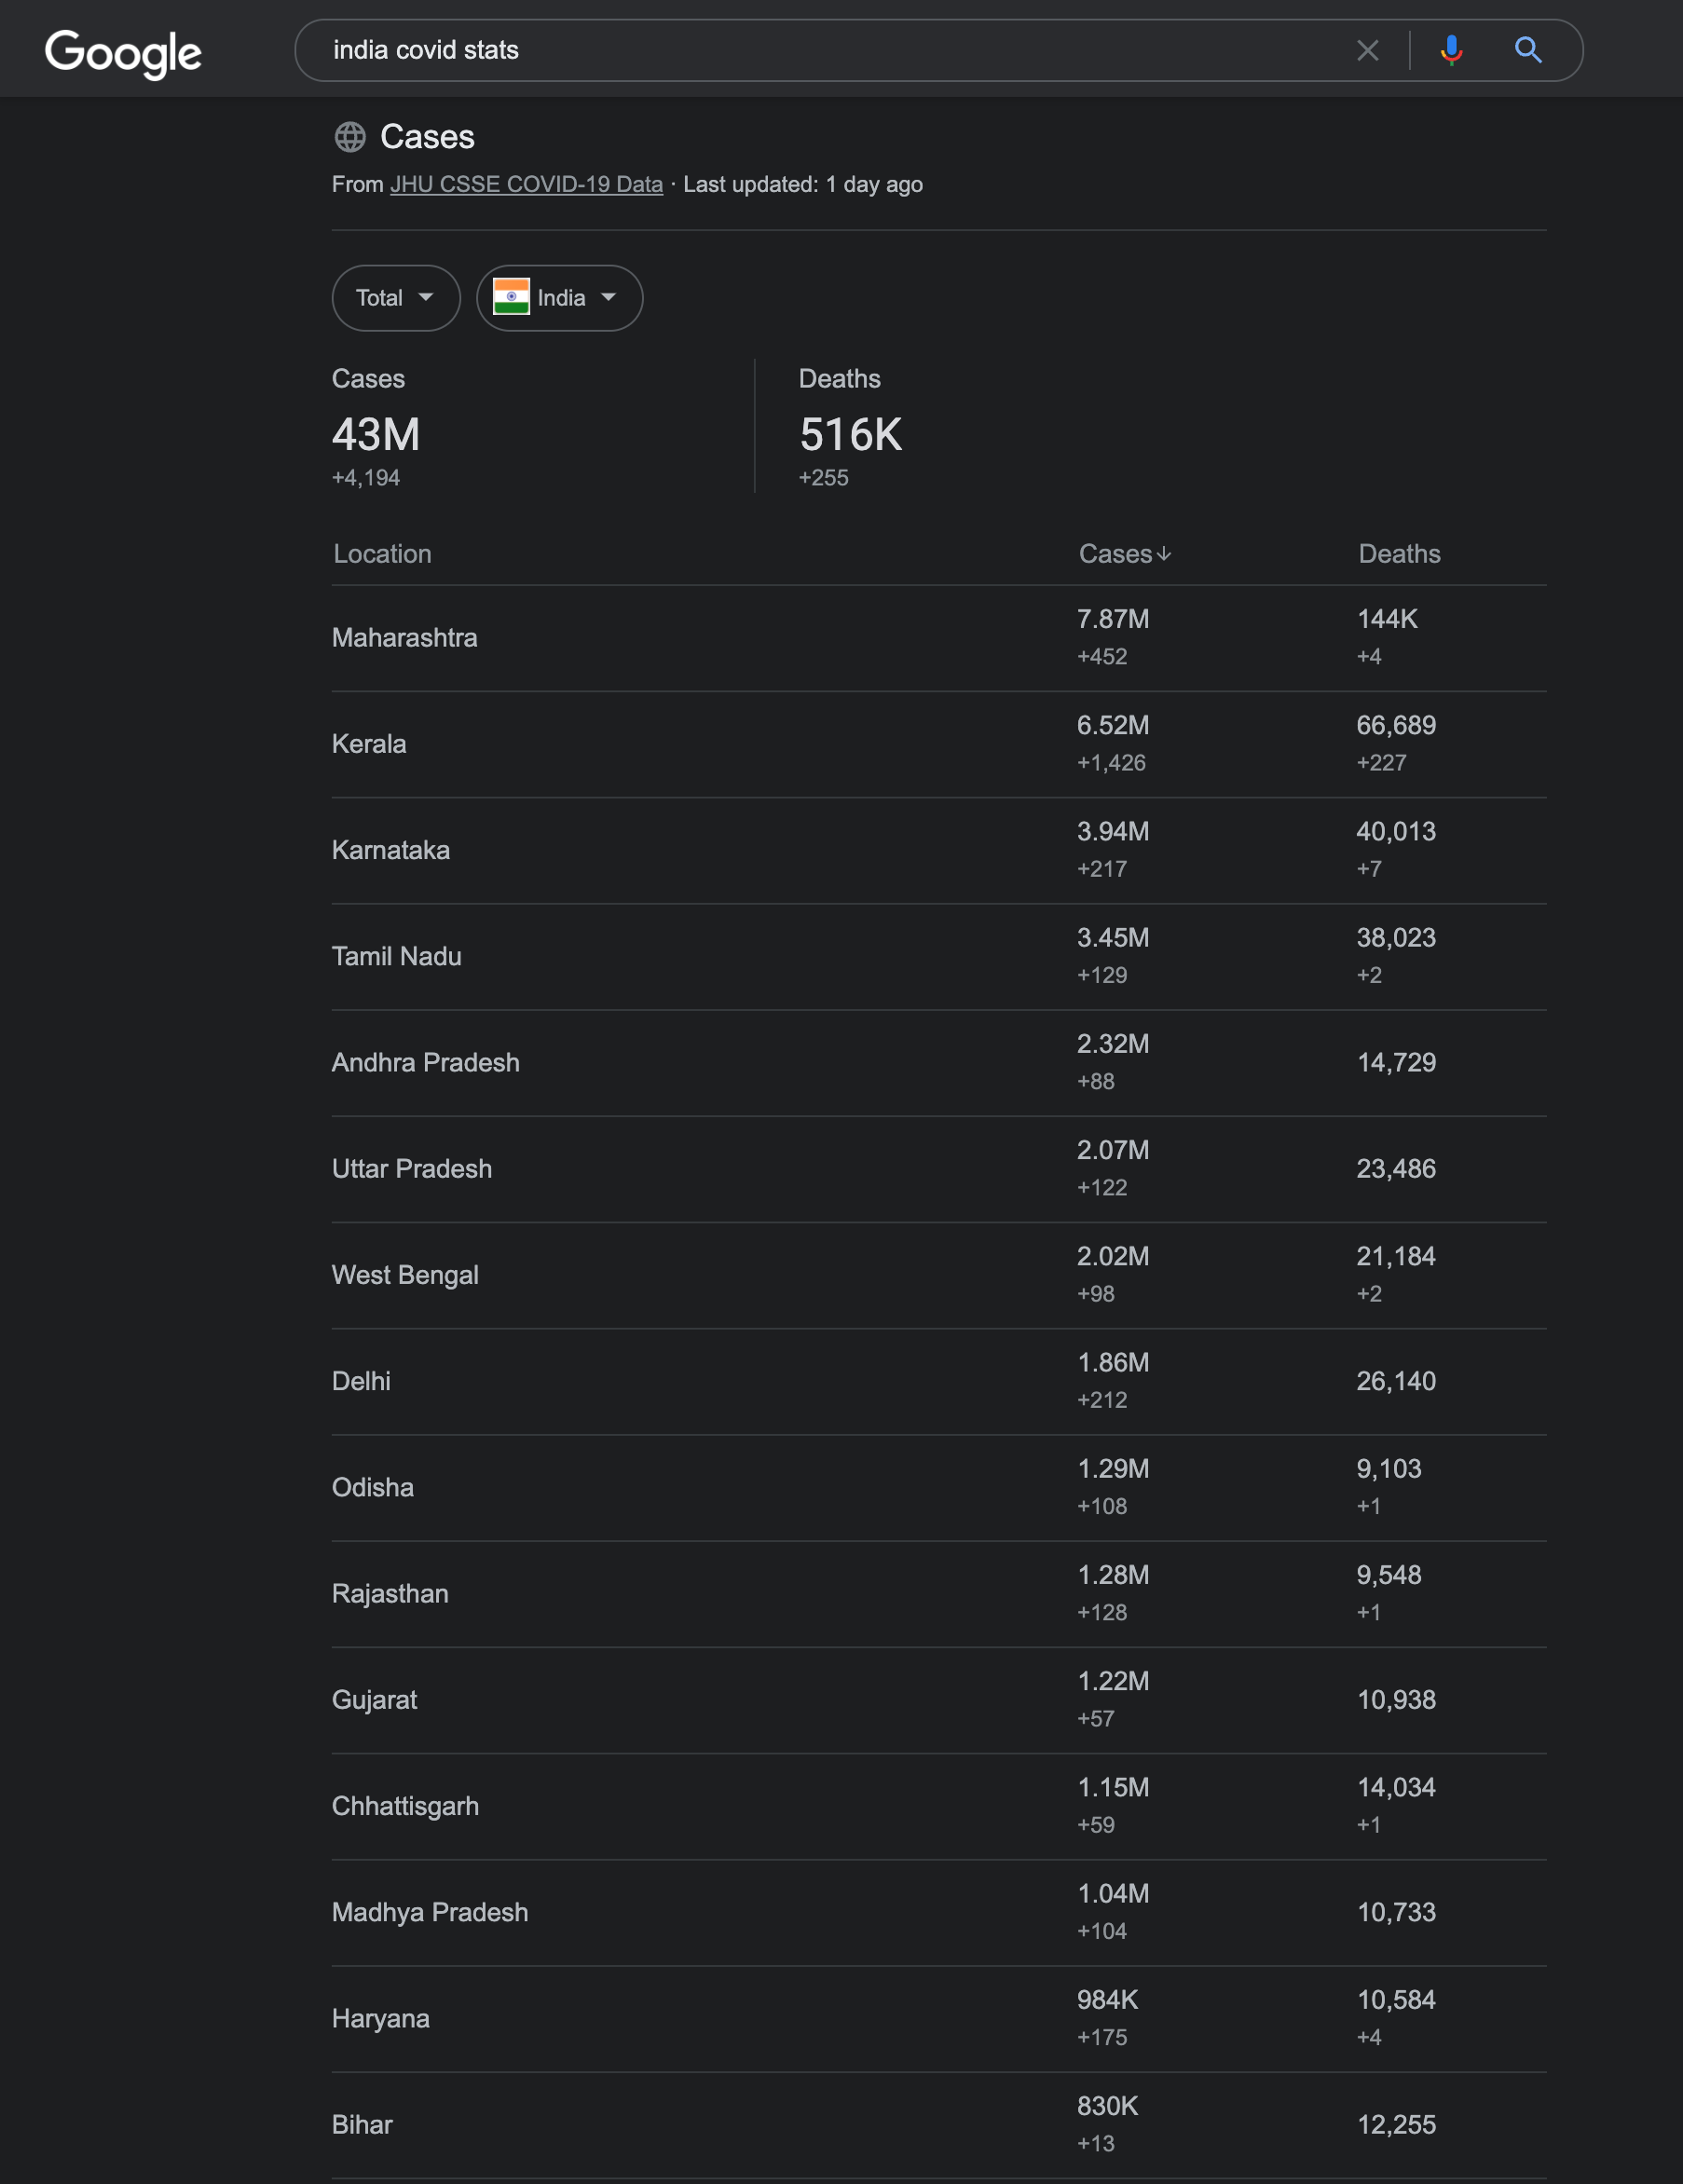
\includegraphics[width=0.7\textwidth]{india-states-mortality}
%    \caption{Cumulative mortality in individual Indian states (March 12, 2022)}
%    \label{fig:india-states-mortality}
%\end{figure}

\begin{figure}[h]
    \centering
    \fbox{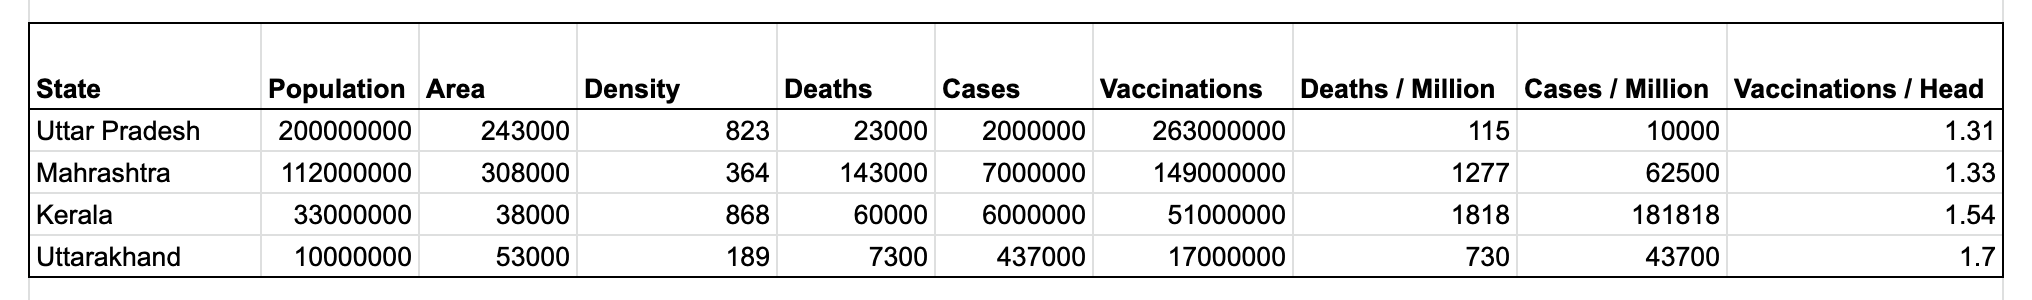
\includegraphics[width=1\textwidth]{india-stats-trunc}}
    \caption{Statistics by state (Febuary 12, 2022), vaccination numbers obtained from \cite{statistaIndiaVaccination}, deaths and cases obtained from \href{https://github.com/CSSEGISandData/COVID-19}{JHU CSSE COVID-19 Data} (Google visualisation). Populations and area from Wikipedia. 13 fold mortality difference between the two most populous states in India, with population density, herd immunity (approximated by number of cases) and vaccination discounted as explanations.}
    \label{fig:india-stats}
\end{figure}

\begin{figure}[h]
    \centering
    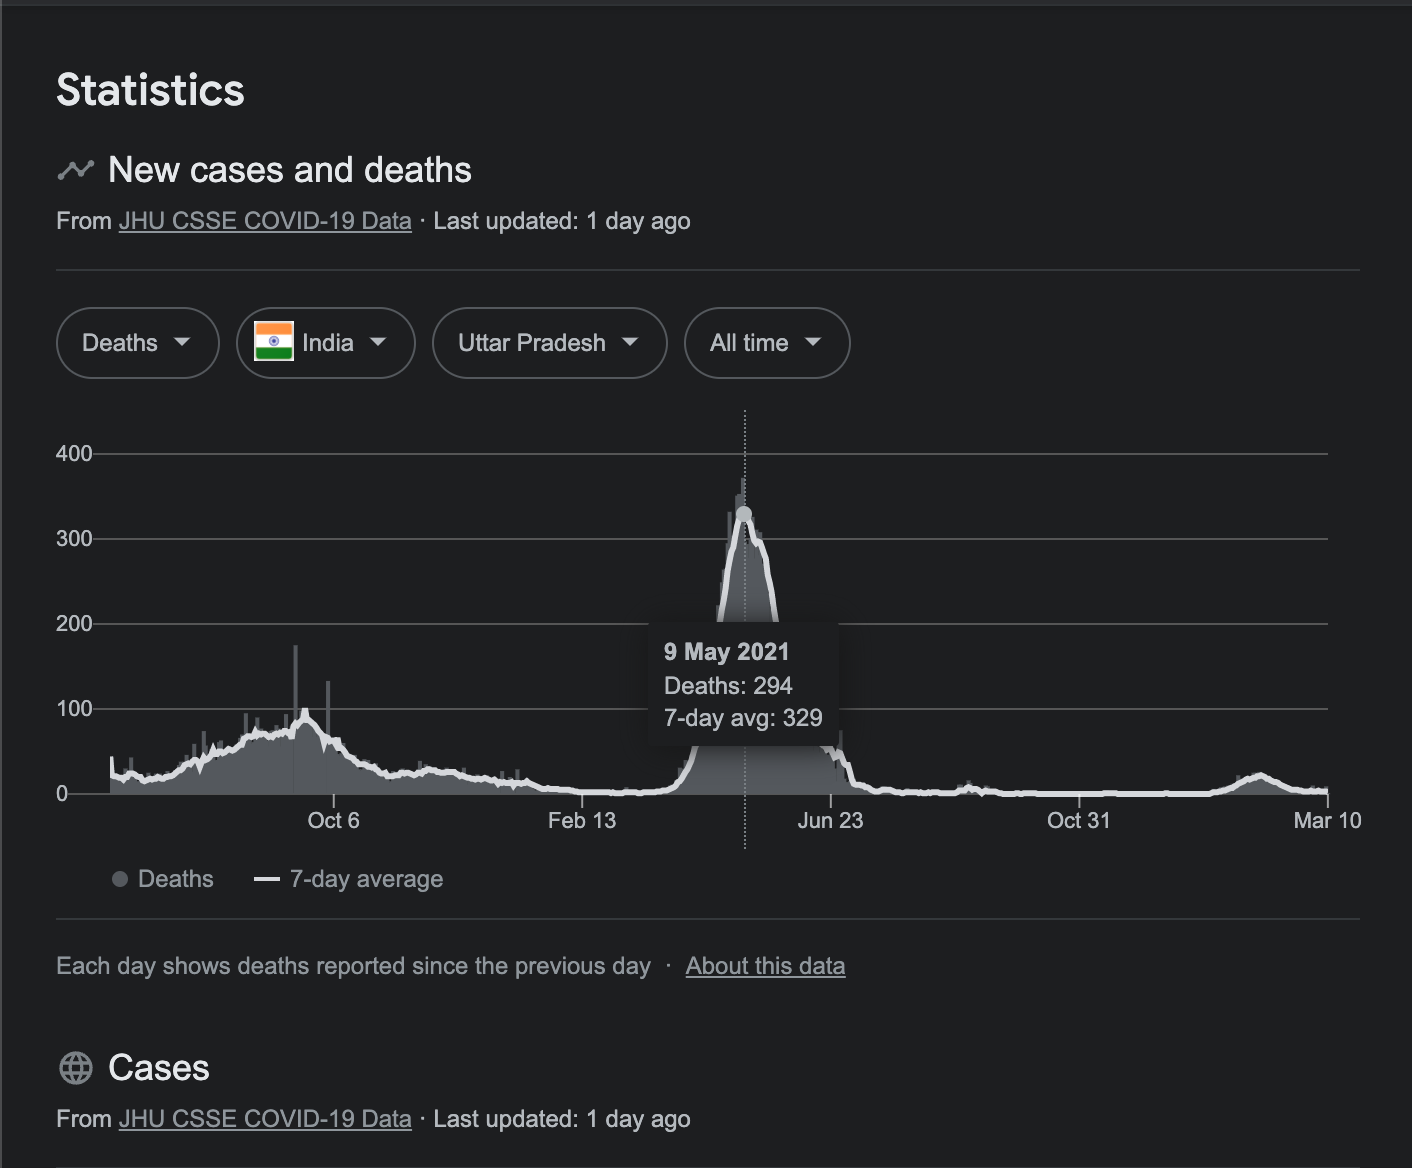
\includegraphics[width=0.7\textwidth]{india-uttarpradesh-mortality}
    \caption{Uttar Pradesh mortality from \href{https://github.com/CSSEGISandData/COVID-19}{JHU CSSE COVID-19 Data} (Google visualisation)}
    \label{fig:india-uttarpradesh-mortality}
\end{figure}

\begin{figure}[h]
    \centering
    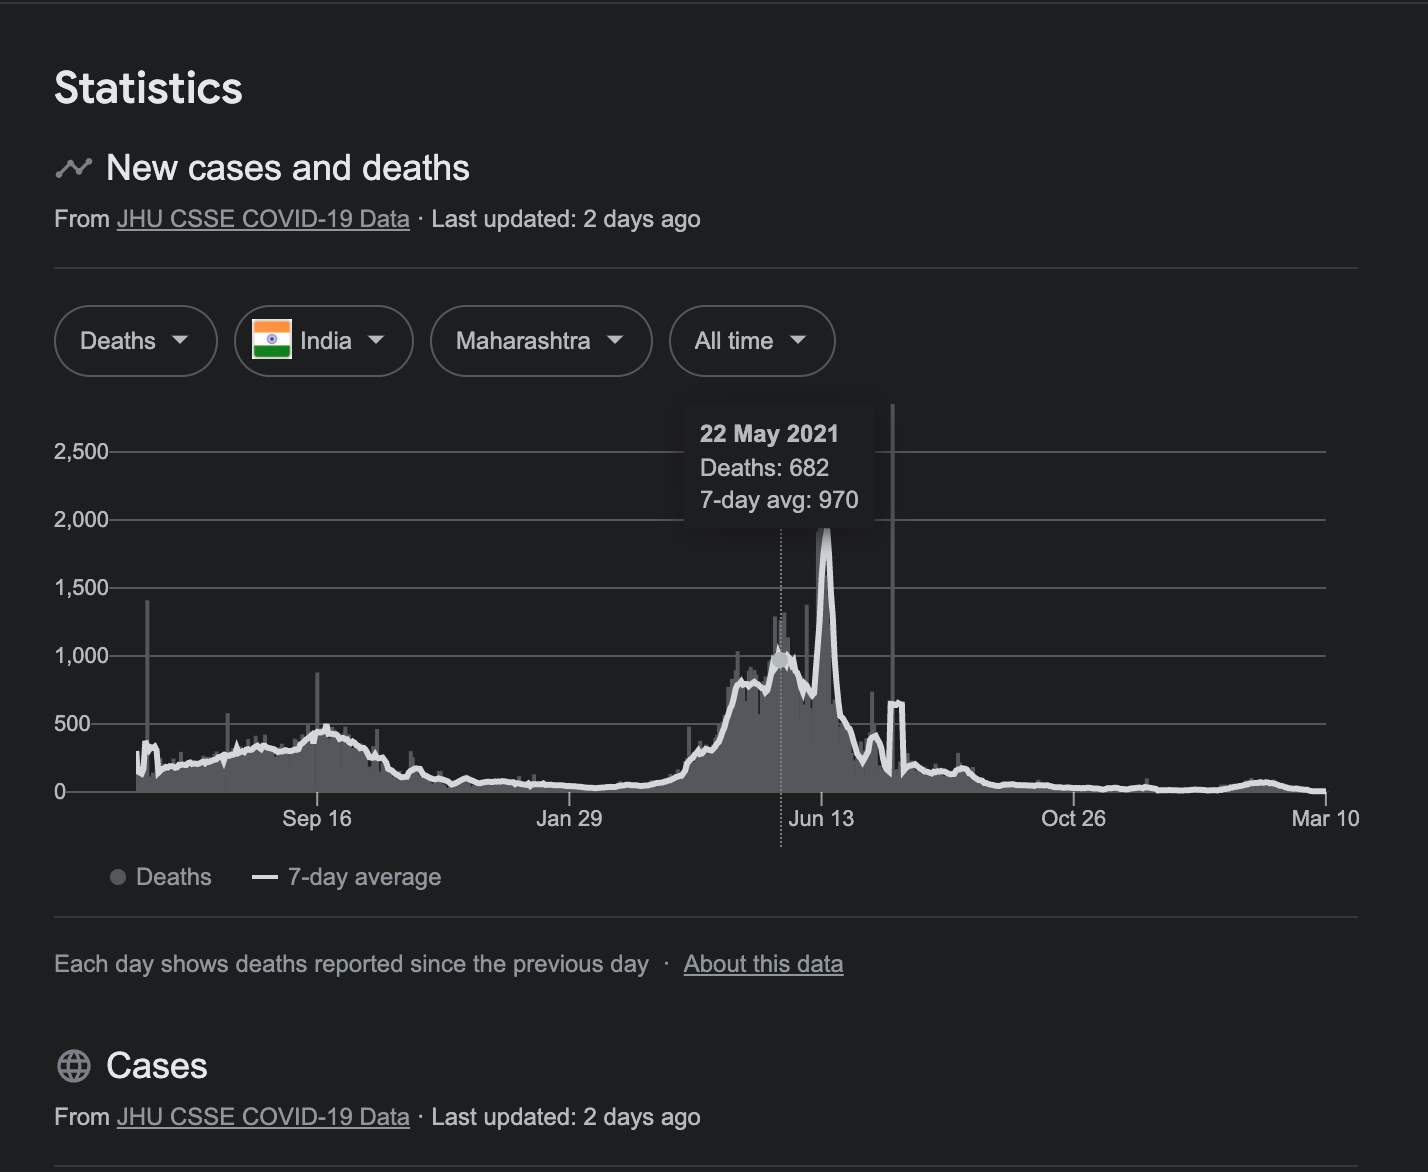
\includegraphics[width=0.7\textwidth]{india-maharashtra-mortality}
    \caption{Maharashtra mortality from \href{https://github.com/CSSEGISandData/COVID-19}{JHU CSSE COVID-19 Data} (Google visualisation)}
    \label{fig:india-maharashtra-mortality}
\end{figure}

\begin{figure}[h]
    \centering
    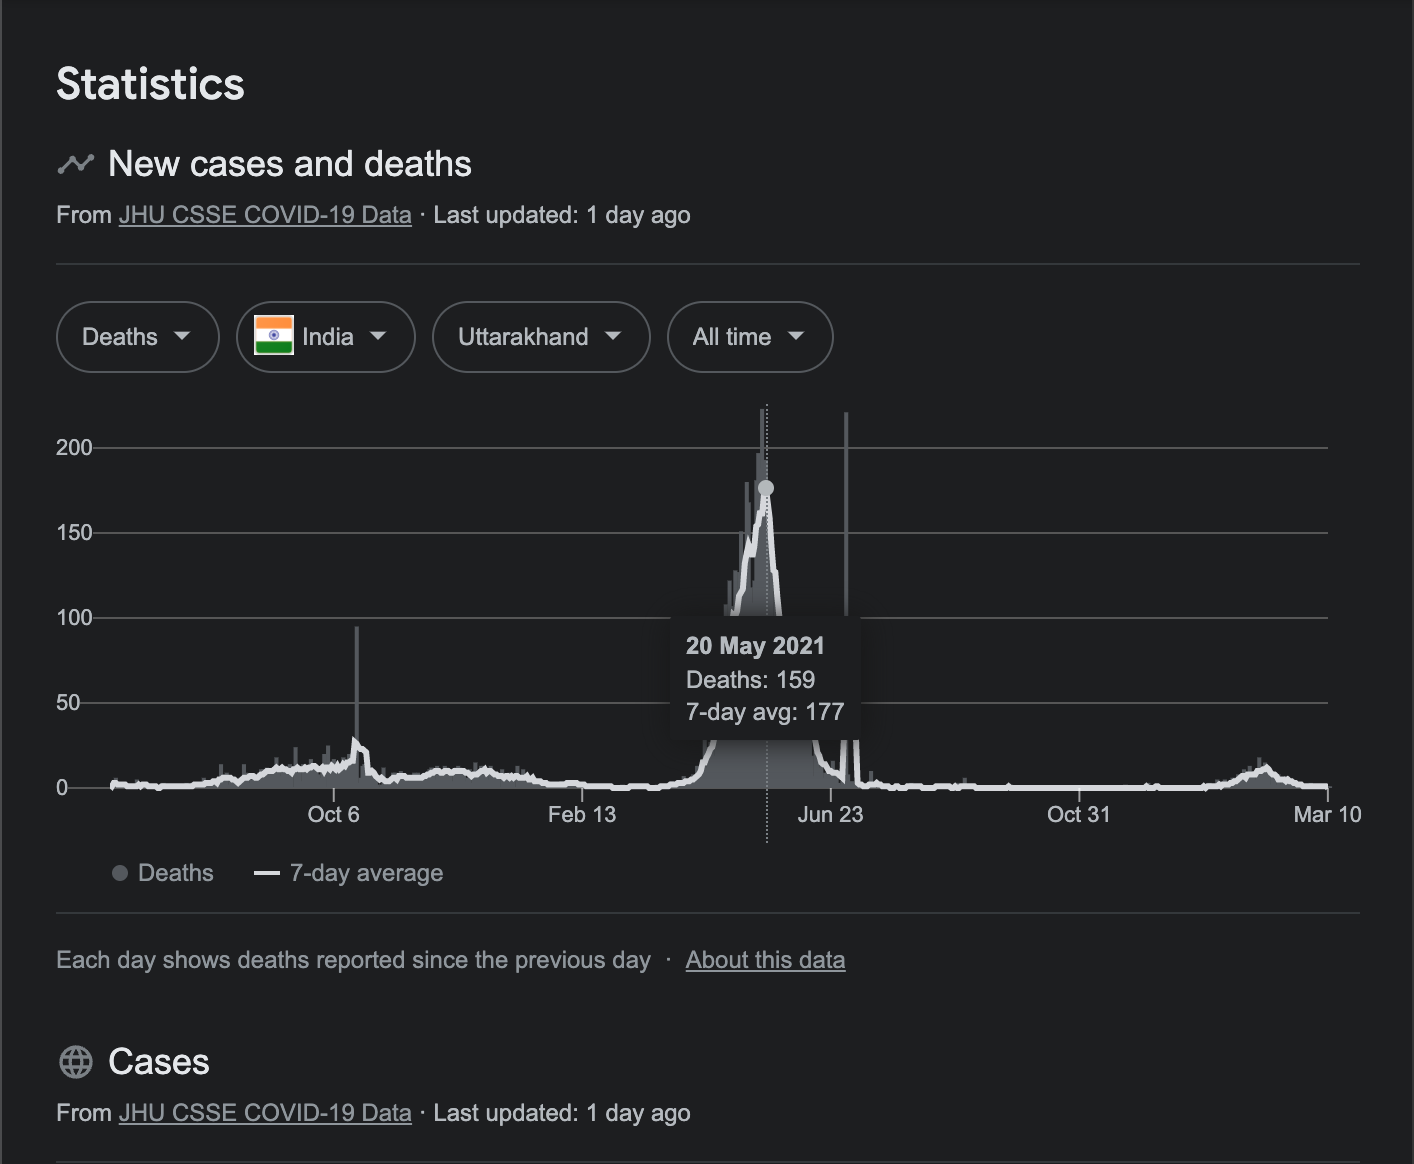
\includegraphics[width=0.7\textwidth]{india-uttarakhand-mortality}
    \caption{Uttarakhand mortality from \href{https://github.com/CSSEGISandData/COVID-19}{JHU CSSE COVID-19 Data} (Google visualisation). The Uttarakhand government started widespread distribution of ivermectin \href{https://economictimes.indiatimes.com/news/india/covid-19-ivermectin-tablets-to-be-distributed-among-uttarakhand-residents-says-state-govt/articleshow/82572159.cms}{on May 14th} \cite{economictimes12052021}, this was followed by an unnaturally steep looking drop in mortality.}
    \label{fig:india-uttarakhand-mortality}
\end{figure}

\begin{figure}[h]
    \centering
    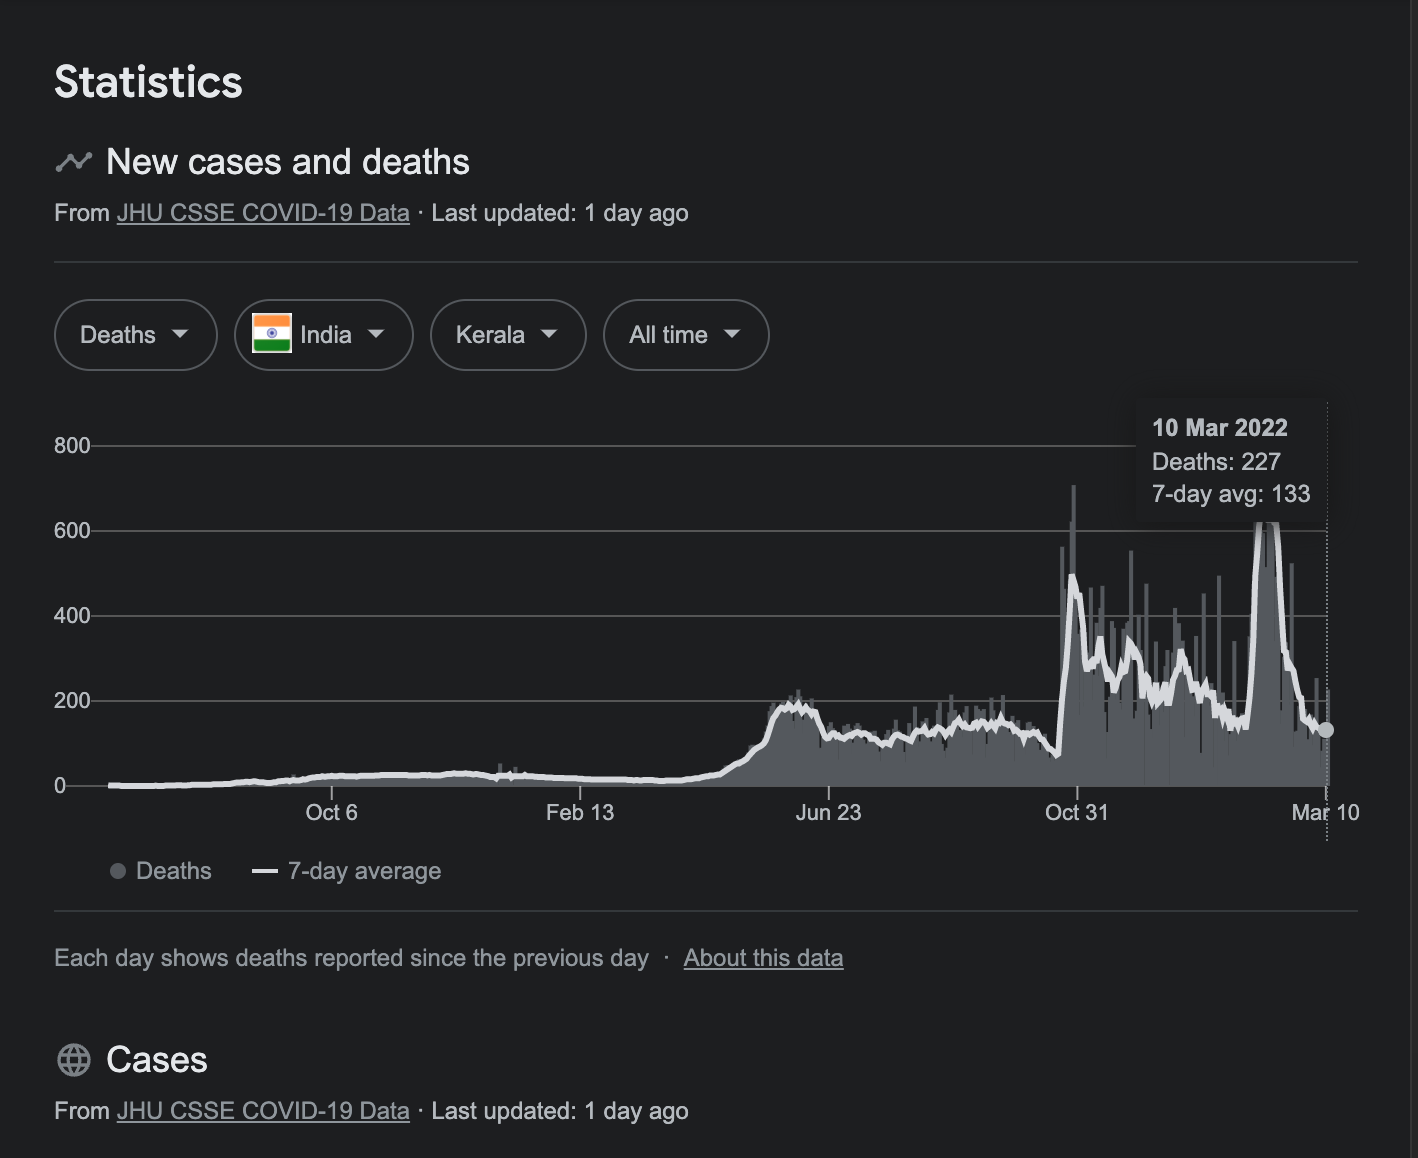
\includegraphics[width=0.7\textwidth]{india-kerala-mortality}
    \caption{Kerala mortality from \href{https://github.com/CSSEGISandData/COVID-19}{JHU CSSE COVID-19 Data} (Google visualisation source). Kerala was \href{https://dhs.kerala.gov.in/wp-content/uploads/2021/04/Kerala-State-COVID-19-guidelines-Version-3.pdf}{using Ivermectin up to summer 2021} \cite{keralagov24042021} then \href{https://www.thehindu.com/news/national/kerala/kerala-revises-covid-19-treatment-guidelines/article35775373.ece}{dropped} their protocol it in favour Remdesivir in the summer of 2021 \cite{hindu06082021}.}
    \label{fig:india-kerala-mortality}
\end{figure}

\clearpage

\subsection*{COVID-19 study in Peru}

\begin{figure}[h]
    \centering
    \fbox{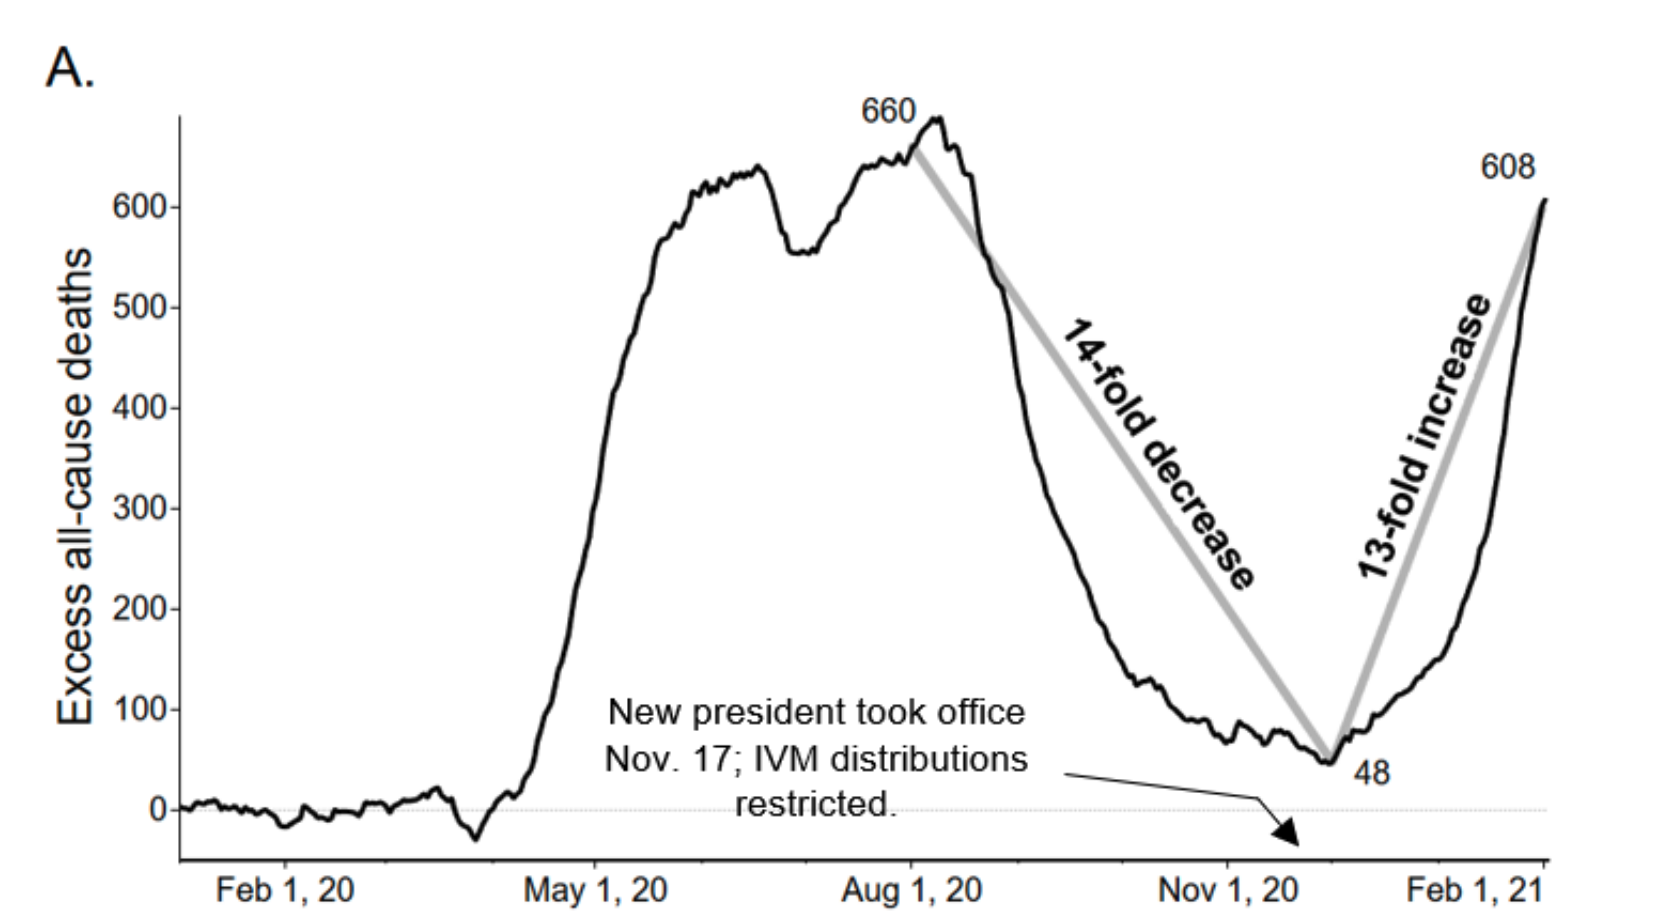
\includegraphics[width=0.7\textwidth]{peru-mortality}}
    \caption{From \citet{Chamie2021}. Peru mortality for over 60 year olds 14-fold Reduction following the introduction of ivermectin followed by 13-fold increase after ivermectin use was restricted.}
    \label{fig:peru-mortality}
\end{figure}

\begin{figure}[h]
    \centering
    \fbox{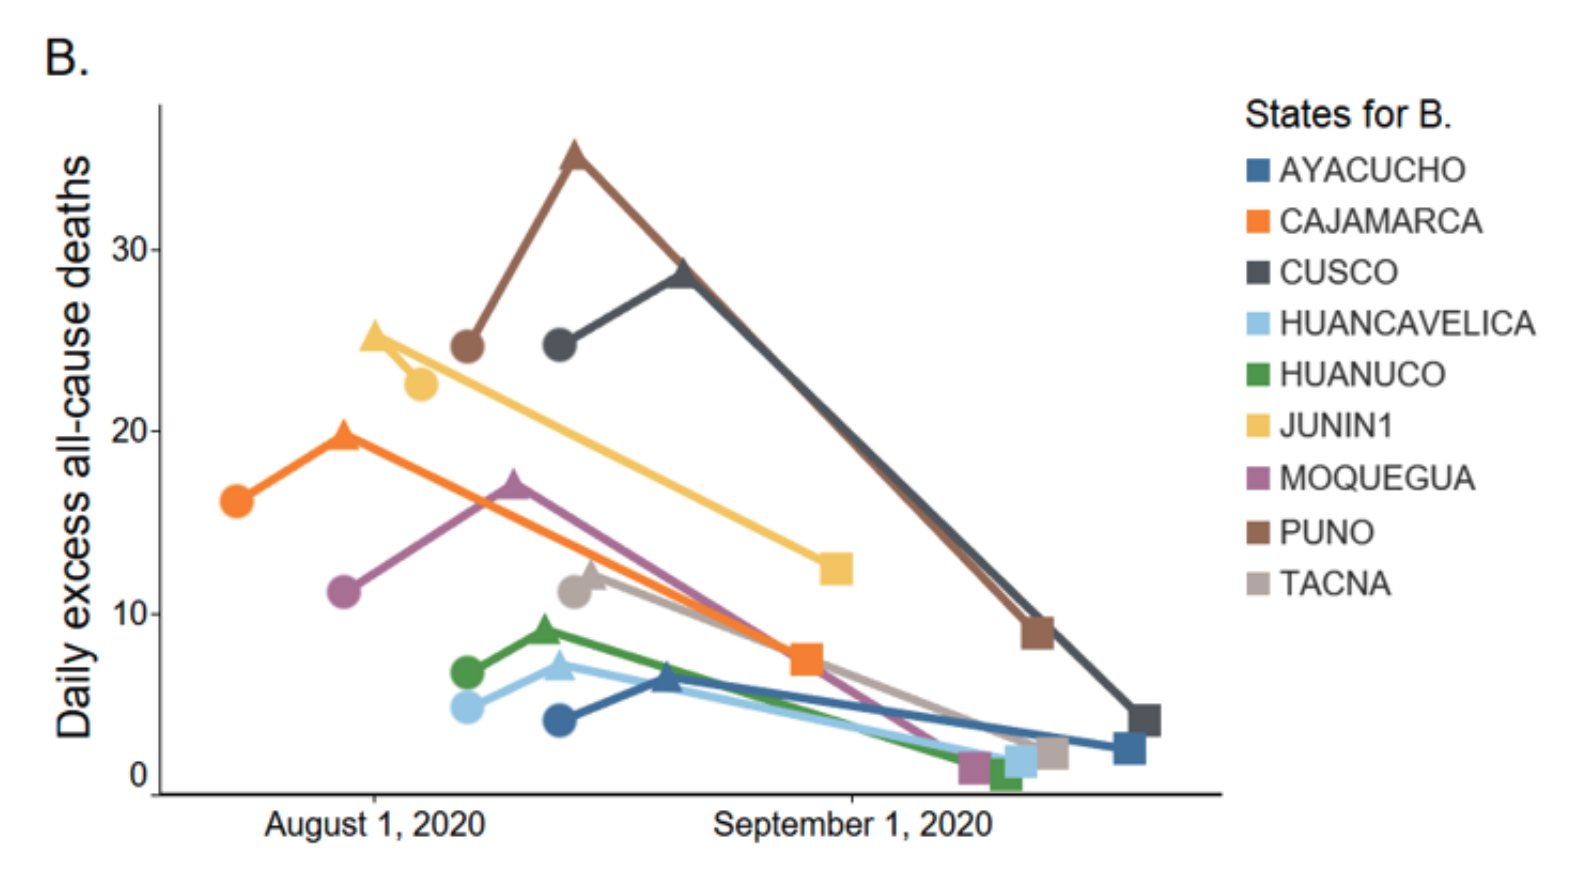
\includegraphics[width=0.7\textwidth]{peru-operation-mot}}
    \caption{From \citet{Chamie2021}. Mortality for each of the 10 Peruvian state covered by operation MOT, an army-led program of mass ivermectin distributions. Circle : MOT start date. Triangle: peak deaths. Square: day of peak deaths + 30 days.}
    \label{fig:peru-operation-mot}
\end{figure}

\clearpage

\subsection*{Worldwide repurposed off-patent usage}

\begin{figure}[h]
    \centering
    \fbox{\includegraphics[width=0.73\textwidth]{hydroxychloroquine-countries}}
    \caption{Countries based on HCQ/CQ usage. From https://c19hcq.com/countries.html}
    \label{fig:hydroxychloroquine-countries}
\end{figure}

\begin{figure}[h]
    \centering
    \fbox{\includegraphics[width=0.73\textwidth]{ivermectin-countries}}
    \caption{Countries based on IVM usage. From https://ivmstatus.com/}
    \label{fig:ivermectin-countries}
\end{figure}

\clearpage

\subsection*{Pfizer safety and efficacy data}

\begin{figure}[h]
    \centering
    \fbox{\includegraphics[width=0.98\textwidth]{Pfizer-6-month-appendix}}
    \caption{Source: supplementary appendix \cite{doi:10.1056/NEJMoa2110345-appendix} of Pfizer's 6 month safety and efficacy assessment \cite{doi:10.1056/NEJMoa2110345}}
    \label{fig:Pfizer-6-month-appendix}
\end{figure}

\clearpage

\subsection*{CDC data visualisations}

\begin{figure}[h]
    \centering
    \fbox{\includegraphics[width=0.98\textwidth]{CDC-natural-immunity}}
    \caption{Immunity through prior infection is superior to vaccine immunity. Data from \href{https://www.cdc.gov/mmwr/volumes/71/wr/mm7104e1.htm}{CDC website} \cite{cdc28012020}}
    \label{fig:CDC-natural-immunity}
\end{figure}

\clearpage

\subsection*{Booster effectiveness against Omicron}

\begin{figure}[h]
    \centering
    \fbox{\includegraphics[width=0.7\textwidth]{Omicron-vaccine}}
    \caption{Booster effectiveness against Omicron, negative from 90 days onward (-76\% for Pfizer, -39\% for Moderna). From \citet{Hansen2021.12.20.21267966}.}
    \label{fig:Omicron-vaccine}
\end{figure}

%\begin{figure}[h]
%    \centering
%    \fbox{\includegraphics[width=0.98\textwidth]{UK-report-w5}}
%    \caption{COVID-19 vaccine \href{https://assets.publishing.service.gov.uk/government/uploads/system/uploads/attachment_data/file/1052353/Vaccine_surveillance_report_-_week_5.pdf}{surveillance report} Week 5 \cite{ukhsa17022022}. Vaccine absolute death risk reduction for under 50 year olds is between 0\% and 0.0025\%.}
%    \label{fig:UK-report-w5}
%\end{figure}

\begin{figure}[h]
    \centering
    \fbox{\includegraphics[width=0.98\textwidth]{UK-report-w11}}
    \caption{COVID-19 vaccine \href{https://assets.publishing.service.gov.uk/government/uploads/system/uploads/attachment_data/file/1061532/Vaccine_surveillance_report_-_week_11.pdf}{surveillance report} Week 11 \cite{ukhsa17032022}. Vaccine absolute death risk reduction for under 50 year olds is between 0\% and 0.0005\%. Negative vaccine effectiveness against Omicron infection aligned with \citet{Hansen2021.12.20.21267966} (Figure \ref{fig:Omicron-vaccine})}
    \label{fig:UK-report-w11}
\end{figure}



%\href{https://www.cdc.gov/mmwr/volumes/71/wr/mm7104e1.htm}{CDC website}
%\cite{cdc28012020}
%Retraction
%https://journals.plos.org/plosone/article?id=10.1371/journal.pone.0258935

%Ridicule of outpatient care 
%https://abcnews.go.com/Health/controversial-doctor-group-touts-ivermectin-long-covid-treatment/story?id=82967318

%Gilead complaint
%https://www.gilead.com/-/media/gilead-corporate/files/pdfs/company-statements/gilead-statement-on-solidarity-trial-final-clean.pdf?la=en

%Remdesevir outpatient
%https://www.fda.gov/news-events/press-announcements/fda-takes-actions-expand-use-treatment-outpatients-mild-moderate-covid-19

%Gilead profits
%https://www.beckershospitalreview.com/pharmacy/gilead-saw-5-6b-in-remdesivir-sales-last-year.html

%RTU refusée
%https://ansm.sante.fr/actualites/lansm-publie-sa-decision-sur-la-demande-de-rtu-pour-livermectine-dans-la-prise-en-charge-de-la-maladie-covid-19

%Guardian saying tabloids are propaganda
%https://www.theguardian.com/environment/climate-consensus-97-per-cent/2017/feb/13/this-is-why-conservative-media-outlets-like-the-daily-mail-are-unreliable

 \bibliographystyle{ametsoc2014}
 \bibliography{main}

\end{document}


